\PassOptionsToPackage{pdfa,pdfapart=1,pdfaconformance=b}{hyperref}
\documentclass[sigconf,review,anonymous]{acmart}

%! TEX root = diffusr.tex
% Keep the list in alphabetical order, unless is really helpful to break it =)
\usepackage{accents} % to use custom accents
\usepackage[ruled,vlined,linesnumbered]{algorithm2e}
\usepackage{cleveref}
\crefname{algorithm}{Alg.}{Algs.}
\Crefname{algorithm}{Algorithm}{Algorithms}
\crefname{appendix}{App.}{App.}
\Crefname{appendix}{Appendix}{Appendices}
\crefname{corollary}{Corol.}{Corolls.}
\Crefname{corollary}{Corollary}{Corollaries}
\crefname{conjecture}{Conjecture}{Conjectures}
\Crefname{conjecture}{Conjecture}{Conjectures}
\crefformat{conjecture}{Conjecture~#2#1#3}
\crefmultiformat{conjecture}{Conjectures~#2#1#3}{\ and~#2#1#3}{, #2#1#3}{\ and~#2#1#3}
\crefname{definition}{Def.}{Defs.}
\Crefname{definition}{Definition}{Definition}
\crefname{figure}{Fig.}{Figs.}
\Crefname{figure}{Figure}{Figures}
\crefname{lemma}{Lemma}{Lemmas}
\Crefname{lemma}{Lemma}{Lemmas}
\crefname{proposition}{Prop.}{Props.}
\Crefname{proposition}{Proposition}{Propositions}
\Crefname{section}{Section}{Sections}
\crefname{section}{Sect.}{Sect.}
\crefname{subsection}{Sect.}{Sect.}
\Crefname{subsection}{Section}{Sections}
\crefname{subsubsection}{Sect.}{Sect.}
\Crefname{subsubsection}{Section}{Sections}
\crefname{table}{Table}{Tables}
\Crefname{table}{Table}{Tables}
\crefname{theorem}{Thm.}{Thms.}
\Crefname{theorem}{Theorem}{Theorems}
\usepackage{dsfont} % for font for indicator function
\usepackage{mathtools} % for DeclarePairedDelimiter, underbracket, …
\usepackage{graphicx} % package for images
\graphicspath{ {./images/} } % path for images
\usepackage{multirow} % for multi-line rows in tables
\usepackage{tikz} % for drawing a custom accent
\usetikzlibrary{decorations.pathmorphing}
\usepackage{xfrac} % for nice inline fractions
\usepackage[font=small,labelfont=bf,labelsep=space]{caption}
\usepackage[font=small,labelfont=bf]{subcaption} % for subfigures

%\usepackage{chato-notes} % temporary package. Remove/comment out before submission

%! TEX root = diffusr.tex
% Keep the list in alphabetical order, unless is *really* helpful to break it =)
\DeclarePairedDelimiter\abs{\lvert}{\rvert} % absolute value
% Swap the definition of \abs*, so that \abs
% resizes the size of the bars, and the starred version does not.
\makeatletter
\let\oldabs\abs%
\def\abs{\@ifstar{\oldabs}{\oldabs*}}
\makeatother
\newcommand{\algoname}{DiFfuSR} % our algorithm name in plain text
\newcommand{\algo}{\textsc{\algoname}} % algorithm name in smallcaps
\newcommand{\arsd}[1]{ARSD(#1)} % average relative support difference of the sampled dataset #1 % chktex 36
\newcommand{\naivealgo}{\textsc{\algoname-N}} % naive algorithm
\newcommand{\refalgo}{\textsc{\algoname-R}} % refined algorithm
\newcommand{\card}[1]{\abs{#1}} % cardinality of a set
\newcommand{\colsnum}{n} % number of columns in dataset
\newcommand{\cols}{C} % set of columns / column vertices
\newcommand{\colsum}[1]{c_#1} % sum of column at index #1 of dataset
\newcommand{\copiesnum}[1]{\mathsf{c}\lparen#1\rparen} % no. of matrices corresponding to dataset #1
\newcommand{\dataset}{\datasetsym} % dataset
\newcommand{\datasetadj}{\datasetsym^\prime} % adjacent dataset
\newcommand{\datasetsym}{\mathcal{D}} % symbol for dataset
\newcommand{\dpairsnum}[1]{\mathsf{J}\lparen#1\rparen} % number of disjoint pairs of edges of graph #1
\newcommand{\expectation}[2]{\mathbb{E}_{#2}\left[#1\right]} % expectation of r.v. #1 w.r.t distribution #2
\newcommand{\fis}[2]{\mathsf{FI}_{#2}(#1)} % frequent itemsets in dataset #2 wrt to threshold #1 % chktex 36
\newcommand{\gioalgo}{\textrm{GMMT}} % name for Gionis et al.'s algo
\newcommand{\hashmap}[1]{\hashmapsym[#1]} % hashmap value for key #1
\newcommand{\hashmapsym}{\mathsf{M}} % symbol for hashmap
\newcommand{\indic}[1]{\mathds{1}[#1]} % indicator function
\newcommand{\items}{\mathcal{I}} % alphabet of items
\newcommand{\kttsnum}[1]{\kttnumsym(#1)} % number of K_{2, 2} cliques of graph #1
\newcommand{\ktt}{\kttnumsym_{2, 2}} % K_{2, 2} clique
\newcommand{\kttnumsym}{\mathsf{K}} % symbol for K_{2, 2} clique
\newcommand{\matrices}{\mathcal{M}} % Set of matrices considered by Gionis et al.'s algo
\newcommand{\mattodat}[1]{\mathsf{dat}\lparen#1\rparen} % function to map matrices to datasets
\newcommand{\neighprob}{\eta} % distribution over the out-neighbors of a state
\newcommand{\newsym}{\prime} % symbol for new object
\newcommand{\nullmodel}{\Pi} % null model
\newcommand{\nullprob}{\pi} % null probability distribution
\newcommand{\nullset}{\mathcal{Z}} % null set of datasets
\newcommand{\odataset}{\smash{\nonsmashedodataset}} % observed dataset
\newcommand{\nonsmashedodataset}{\mathring{\dataset}}
\newcommand{\population}{\mathcal{P}} % population from which to sample
\newcommand{\pval}[2]{\mathsf{p}_{#1}\lparen#2\rparen} % p-value of pattern #2 in dataset #1
\newcommand{\epval}[2]{\tilde{\mathsf{p}}\lparen#1, #2\rparen} % estimate of p-value dataset #1 using the set of datasets #2
\newcommand{\rowsnum}{m} % number of rows in the dataset
\newcommand{\rows}{R} % set of rows / row vertices
\newcommand{\rowsum}[1]{r_{#1}} % sum of row at index #1 of dataset
\newcommand{\samplprob}{\xi} % sampling distribution for \population
\newcommand{\selfspairsnum}[1]{\mathsf{H}\lparen#1\rparen} % number of swaps from a dataset to itself
\newcommand{\spairsnum}[2]{\mathsf{sw}_{#1}\lparen#2\rparen} % number of swaps from dataset #1 to #2
\newcommand{\spairs}{\mathcal{G}} % set of swaps from a dataset to another
\newcommand{\spairsfactor}{\chi} % correcting factor for the number of swaps
\newcommand{\squaredmat}{Q} % Product of the matrix representation of a dataset by its transpose
\newcommand{\sumtlen}{w} % sum of the transaction lengths
\newcommand{\supp}[2]{\sigma_{#1}(#2)} % support of itemset #1 in dataset #2 % chktex 36
\newcommand{\states}{\mathcal{S}} % state space of Markov chain
\newcommand{\statprob}{\zeta} % stationary distribution for a Markov chain
\newcommand{\suchthat}{\mathrel{:}} % "such that" symbol for set definitions, with the right spacing
\newcommand{\swapnum}{s} % number of swaps
\newcommand{\swapnummult}{k} % swap number multiplier
\newcommand{\thresh}{\theta} % minimum support threshold
\newcommand{\titlefirstpart}{Distortion-Free Swap-Randomization}
\newcommand{\titlesecondpart}{for Statistically-Testing Data Mining Results}
\newcommand{\totspairsnummat}[1]{\mathsf{mts}\lparen#1\rparen} % total number of possible swaps for matrix #1
\newcommand{\totspairsnumdat}[1]{\mathsf{dts}\lparen#1\rparen} % total number of possible swaps for matrix #1
\newcommand{\uniform}[1]{\mathcal{U}\lparen#1\rparen} % uniform distribution over the set #1
\newcommand{\zstructsnum}[1]{\zstructsnumsym(#1)} % number of Z structures of graph #1
\newcommand{\zstructsnumsym}{\mathsf{Z}} % symbol for number of Z structures

\newsavebox\wigglybox%
\savebox\wigglybox{%
\begin{tikzpicture}[line width=0.15pt,smooth]
  \draw[semithick,decoration={zigzag,segment length=1.2,amplitude=.3},decorate]
    (0,0) -- (0.15,0);
\end{tikzpicture}%
}
\newcommand\wiggly[1]{\accentset{\mathbin{\usebox\wigglybox}}{#1}}


\copyrightyear{2022}
\acmConference[KDD '22]{28th ACM SIGKDD Conference on Knowledge Discovery and
Data Mining}{August 14--18, 2022}{Washington, DC, USA}
\setcopyright{rightsretained}
% 20220129 MR: temporary to avoid an overfull hbox
\acmDOI{10.1145/nnnnn.nnnnn}

\begin{document}

\title[\algoname: \titlefirstpart\ \titlesecondpart]{\texorpdfstring{\algoname: \titlefirstpart\\ \titlesecondpart}{\algoname: \titlefirstpart\ \titlesecondpart}}
% Other title ideas:
% Mining Statistically Significant Itemsets\\with Distortion-free Swap Randomization
% Mining Statistically Significant Itemsets without Distortion

\author{Alexander Lee}
\affiliation{%
  \department{Department of Computer Science}
  \institution{Amherst College}
  \streetaddress{Box \#2232, Amherst College}
  \city{Amherst}
  \state{MA}
  \postcode{01002}
  \country{USA}
}
\email{awlee22@amherst.edu}

\author{Matteo Riondato}
\orcid{0000-0003-2523-4420} %chktex 8
\affiliation{%
  \department{Department of Computer Science}
  \institution{Amherst College}
  \streetaddress{Box \#2232, Amherst College}
  \city{Amherst}
  \state{MA}
  \postcode{01002}
  \country{USA}
}
\email{mriondato@amherst.edu}

\begin{teaserfigure}
  \noindent\textit{``I'm big into aromatherapy''} --- Sharon Stone
  \Description{Not a figure.}
\end{teaserfigure}

\chapter*{Abstract}

We present \algo, a set of algorithms for drawing transactional datasets from
a null model, to be used for the statistical validation of knowledge discovery
results. Our algorithms assume the widely-adopted null model that maintains
transaction lengths and item supports, and they are based on swap
randomization, i.e., randomly swapping items between transactions, in a
Markov-Chain Monte-Carlo (MCMC) setting, using Metropolis-Hastings. In contrast
with previous work, our approach does not suffer from the distortion of the null
space introduced by identifying the set of transactional datasets with the set
of binary matrices, which could lead to unknown false positives in the output.
\algo\ uses carefully-designed Markov chains with appropriate stationary
distributions to sample datasets from the null model. The results of our
experimental evaluation show that \algo\ solves the distortion issue, is fast
and (empirically) rapidly-mixing, and scales well as the dataset size grows.


\begin{CCSXML}
<ccs2012>
   <concept>
       <concept_id>10002951.10003227.10003351</concept_id>
       <concept_desc>Information systems~Data mining</concept_desc>
       <concept_significance>500</concept_significance>
       </concept>
   <concept>
       <concept_id>10003752.10010061.10010065</concept_id>
       <concept_desc>Theory of computation~Random walks and Markov chains</concept_desc>
       <concept_significance>500</concept_significance>
       </concept>
   <concept>
       <concept_id>10002950.10003648.10003662.10003666</concept_id>
       <concept_desc>Mathematics of computing~Hypothesis testing and confidence interval computation</concept_desc>
       <concept_significance>500</concept_significance>
       </concept>
   <concept>
       <concept_id>10002950.10003648.10003670.10003677.10003679</concept_id>
       <concept_desc>Mathematics of computing~Metropolis-Hastings algorithm</concept_desc>
       <concept_significance>500</concept_significance>
       </concept>
</ccs2012>
\end{CCSXML}

\ccsdesc[500]{Information systems~Data mining}
\ccsdesc[500]{Theory of computation~Random walks and Markov chains}
\ccsdesc[500]{Mathematics of computing~Hypothesis testing and confidence interval computation}
\ccsdesc[500]{Mathematics of computing~Metropolis-Hastings algorithm}

% Separate the keywords with commas.
\keywords{Frequent Patterns, Itemsets, Family-Wise Error Rate}

\maketitle

%! TEX root = diffusr.tex
\section{Introduction}\label{sec:intro}

Knowledge discovery results obtained from a dataset (e.g., patterns,
clusters, anomalies) should be \emph{statistically validated} in order to ensure
that they are not just due to the randomness in the data-generating
process~\citep{GionisMMT07,HamalainenW19,PellegrinaRV19b}: the goal of the
analysis is to \emph{gain knowledge of this process through the observed
dataset}, rather than knowledge of the dataset itself.

One such validation subjects the results to \emph{statistical hypothesis
tests}~\citep[Ch.\ 10]{Wasserman05} (see \cref{sec:prelims:significant}):
results that pass the tests are marked as \emph{(statistically) significant}, as
there is evidence that they give information on the data generating process.

The significance of the results is assessed against a \emph{null model} (see
\cref{sec:prelims:significant}), which is a collection of \emph{possible}
datasets that the unknown process \emph{may} generate, and a probability
distribution over this collection. The null model captures, in some sense, what
is assumed or already known about the data generating process, and the results
are assessed against it to understand in what way they cannot be explained by
the existing knowledge or assumptions.

The choice of the null model made by the user must be \emph{deliberate and informed},
as the meaning of ``statistically significant'' depends on the null model. For
example, the results deemed significant under one null model cannot in general
be compared to those deemed significant under a different null model.
Nevertheless, as the aphorism says: ``all models are wrong, but some are
useful'' (George E.\,P.\ Box), and some null models may be more appropriate for
testing the significance of the results than others, because they more closely
represent the settings of the task. It is therefore important that users have
access to a variety of null models and are informed of the differences between
them, in order to be able to select the more appropriate one for their needs. In
this work, we introduce a null model for testing the significance of results
obtained from \emph{binary transactional datasets}, such as (but not limited to)
collections of frequent itemsets~\citep{AgrawalS94}. A null model is, in some sense,
independent from the task whose results one wants to validate, as a null model
is a set of datasets, not results, but is used to evaluate results. Our model is
more appropriate for evaluating the results of common tasks on transactional
datasets than existing ones~\citep{GionisMMT07}, as we explain in the
\emph{Contributions} paragraph and in \cref{sec:gionis}.

Many statistical hypothesis tests are based on
\emph{resampling}~\citep{WestfallY93}: they analyze multiple datasets drawn
from the null model distribution, in order to approximate the distribution of
the test statistic and compare its value in the observed data against such
distribution. Thus, it is necessary to develop computationally-efficient
procedures for sampling such datasets from the null model distribution.

\paragraph{Contributions} We study the problem of evaluating the significance of
results extracted from unlabeled transactional datasets using resampling-based
statistical hypothesis tests.

\begin{itemize}
  \item We introduce a novel null model that preserves transaction lengths and
    item supports, but does not suffer from  the \emph{distortion} introduced by
    equating the set of datasets and the set of binary matrices (see
    \cref{sec:related,sec:gionis}), and is therefore more appropriate for
    evaluating the results of knowledge discovery tasks on transactional
    datasets. The user can specify \emph{any} distribution over the set of
    datasets.
  \item We present \algo\ (for \emph{Di}stortion-\emph{F}ree
    % 20211117 MR: manual line break in the following line, due to the \emph.
    \emph{S}wap \emph{R}andomiza-\\tion), a set of algorithms for sampling datasets
    from the null model we introduce. Our algorithms are based on
    \emph{swap-randomization} (\cref{sec:diffusr}). Our algorithms take a
    Markov-Chain Monte-Carlo (MCMC) approach on appropriately-defined Markov
    chains (see \cref{sec:prelims:markov}) over either the set of binary
    matrices (for our ``na\"{\i}ve'' algorithm), or the set of datasets (for our
    ``refined'' algorithm), whose stationary distribution is the user-specified
    sampling distribution.
  \item Our algorithms can be seen as the core of procedures to assess the
    statistical validity of data mining results using a resampling
    approach~\citep{WestfallY93} (see \cref{sec:prelims:significant}). To show
    the usefulness of our algorithms, we focus on the task of evaluating the
    significance of the number of frequent itemsets in a dataset, by
    computing an empirical $p$-value of this statistic.
  \item The results of our experimental evaluation show that the distortion
      issue is very relevant and affects the outcome of the testing of data mining
      results. \algo\ does not suffer from it, while being fast, (empirically)
      rapidly-mixing, and scalable as the dataset grows.
\end{itemize}

%! TEX root = diffusr.tex
\section{Related work}\label{sec:related}

Evaluating the statistical significance of results obtained by mining
transactional datasets has been recognized as important soon after the first
efficient mining algorithms were introduced. For example, \citet{BrinMS97}
use the chi-square test to assess the significance of association rules, while
\citet{MegiddoS98} use statistical significance testing to measure the number of
false discoveries.

Many measures of interestingness, both for individual patterns and for sets of
patterns~\citep{KontonasiosSDB12,TanKS04,VreekenT14}, were introduced with the
goal of mitigating the pattern explosion observed when using frequency as a
proxy of interestingness, but they do not offer the strict statistical
guarantees that allow precise statements about the interestingness of a pattern
w.r.t.\ the data generation process.

The framework of statistical hypothesis testing~\citep[Ch.\ 10]{Wasserman05}
offers such guarantees, and is now the de facto standard taken by works in
statistically-significant pattern mining~\citep{HamalainenW19,PellegrinaRV19b}.
The area of statistical pattern mining can be split into two classes, depending
on whether each transaction in the dataset is associated to a (binary or real)
label. Our method \algo\ works on \emph{unlabeled} datasets thus it can be used
for mining significant patterns in this setting, but many works studied the
labeled
case~\citep{LlinaresLopezSPB15,MinatoUTTS14,PellegrinaV20,PellegrinaRV19a,TeradaOHTS13,WuHGLZY16,KomiyamaIANM17}.
To keep the presentation focused, we only discuss contributions for unlabeled
datasets. The tutorial by \citet{PellegrinaRV19b} offers an in-depth
presentation of the labeled case.

Mining significant patterns requires \emph{testing multiple hypotheses}, one per
pattern. Due to the randomness of the data generation process, and the fact that
one only has access to the observed dataset, it is necessary to accept the
possibility of wrongly marking a pattern as significant even if it is not, i.e.,
of making a \emph{false discovery} involving that pattern, or, equivalently,
that the pattern is a \emph{false positive}. Algorithms for significant pattern
mining must therefore give \emph{probabilistic guarantees} on the presence of
false positives in their output. The most common of such guarantees is a bound
on the \emph{Family-Wise Error Rate (FWER)}, i.e., on the probability that the
output collection contains \emph{any} false positives. In pattern mining,
\citet{Webb06,Webb07}, \citet{Hamalainen10}, \citet{LowKRKP13}, and many others
(see the tutorial by \citet{HamalainenW19}) present methods to control the FWER
using the \emph{Bonferroni correction}~\citep{Bonferroni37}. This approach, even
when refined~\citep{Holm79,Webb08}, does not take into account dependencies and
correlations among hypotheses, i.e., the \emph{structure} of the hypothesis
class, which is very rich for the classes associated to patterns. Additionally,
these classes contain many patterns that would never be marked as significant
(e.g., because they do not appear in the observed dataset), thus using the
Bonferroni correction, while controlling the FWER to the desired level, results
in low statistical power, i.e., in not marking many true significant patterns as
such. One alternative is to control the False Discovery Rate (FDR), i.e., the
expected number of false positives, as proposed by \citet{KirschMPPUV12}. The
FDR is a less stringent guarantee than the FWER, thus is only appropriate in
some settings, while controlling the FWER is required in many cases. Resampling
methods~\citep{WestfallY93} take into account the structure of the hypothesis
class and offer high statistical power, while still bounding the FWER\@. \algo\
is designed to be used in such methods.

The resampling method by \citet{GionisMMT07}, while it can be used as the  core
component of a significant pattern mining algorithm, it is, like our work, more
generic and useful for assessing the validity of data mining results. They
do not discuss controlling the FWER, a void filled by \citet{Hanhijarvi11}.
\citet{GionisMMT07} look at transactional datasets as binary matrices, and
consider the null model composed by \emph{all} such matrices with the same row
and column sums (a.k.a., margins) as the observed dataset. We discuss
\citet{GionisMMT07}'s method in detail in \cref{sec:gionis}. The issue with this
approach that we identify and solve is that the space of matrices with
constrained margins does not actually have a one-to-one correspondence with the
space of transactional datasets with the same transaction lengths and item
frequencies, thus creating a \emph{distortion} of the latter space, and
effectively leading to performing statistical tests w.r.t.\ a \emph{different}
null model. The statistical significance of the observed results depends on the
null model, thus the distortion may make results that are not actually
significant appear as such, and vice versa. Our algorithms are
\emph{distortion-free} and sample w.r.t.\ the intended null model.

The randomization approach by \citet{GionisMMT07} has been extended to other
types of data (database tables~\citep{OjalaGGM10}, real-valued and mixed-value
matrices~\citep{OjalaVKHM08,Ojala10},
graphs~\citep{HanhijarviGP09,GunnemannDJE12}, genomic
data~\citep{FerkingstadHS15}), to different kinds of patterns
(sequences~\citep{TononV19}, subgroups~\citep{DuivesteijnK11}), and to the
iterative setting~\citep{HanhijarviOVPTM09}.  The  distortion issue affecting
\citet{GionisMMT07}'s approach is also present in many of these methods, and our
proposed solution can be adapted to these cases. We discuss some of them in
\cref{sec:extensions}, but due to space limitations, we postpone an in-depth
treatment to the extended version of this work.

%! TEX root = diffusr.tex
\section{Preliminaries}\label{sec:prelims}

We now introduce the main concepts used in the work. To exemplify the
application of \algo, we focus on the task of evaluating whether the size of the
collection of frequent itemsets in an observed dataset is statistically
significant. We choose this task because it allows for a self-contained
presentation that is accessible also to non-experts, rather than describing an
arguably more interesting, but certainly more convoluted task such as mining
statistically-significant frequent patterns. We remark that \algo\ can be used
to validate any kind of results obtained from transactional datasets, including
mining statistically-significant frequent patterns (not necessarily itemsets),
evaluating the correlations between different items, and much more (see also
\cref{sec:extensions}).

Let $\items \doteq \{a_1, \dotsc, a_{\colsnum}\}$ be a finite \emph{alphabet}
of $\colsnum \doteq \card{\items}$ \emph{items}. Without loss of generality, we
can assume $\items = \{1, \dotsc, \colsnum\}$. An \emph{itemset} $A \subseteq
\items$ is any non-empty subset of $\items$. A
\emph{dataset} $\dataset \doteq \{t_1, \dotsc, t_{\rowsnum} \}$ is a finite
\emph{bag} of $\rowsnum \doteq \card{\dataset}$ itemsets which, as the elements
of $\dataset$, are known as \emph{transactions}. An itemset $A$ \emph{appears}
in a transaction $t$ when $A \subseteq t$. The \emph{support
$\supp{\dataset}{A}$ of itemset $A$ in dataset $\dataset$} is the number of
transactions of $\dataset$ in which $A$ appears, i.e.,
\[
  \supp{\dataset}{A} \doteq \card{\{ t \in \dataset \suchthat A \subseteq t \}}
  \enspace.
\]
Given a \emph{minimum support threshold} $\thresh \in [1, \card{\dataset}]$, the
set $\fis{\thresh}{\dataset}$ of \emph{frequent itemsets in $\dataset$ w.r.t.\
$\thresh$} is the set of itemsets that have support at least $\thresh$ in
$\dataset$, i.e.,
\[
  \fis{\thresh}{\dataset} \doteq \left\{ A \subseteq \items, A \neq \emptyset\ :\
    \supp{\dataset}{A} \ge \thresh \right\} \enspace.
\]

\subsection{Null models and significant results}\label{sec:prelims:significant}

Statistical significance is assessed w.r.t.\ a user-specified \emph{null model}.
A null model is, for our purposes, a pair $\nullmodel \doteq (\nullset,
\nullprob)$, where $\nullset$ is a set of datasets,  known as the \emph{null
set}, and $\nullprob$ is a probability distribution over $\nullset$. In the
setting we consider, there is one fixed \emph{observed dataset} $\odataset$, and
the null set $\nullset$ is such that $\odataset \in \nullset$ and $\nullset$
contains all and only datasets that share some characteristic properties with
$\odataset$. Thus, the null model depends on the observed dataset $\odataset$.
We follow all previous work and only consider null models where $\nullset$
contains all and only the datasets $\dataset$ such that
\begin{itemize}
  \item $\card{\dataset} = \card{\odataset} = \rowsnum$, i.e., $\dataset$ has
    the same \emph{size}, i.e., number $\rowsnum$ of transactions, as
    $\odataset$; and
  \item if we let $\dataset=\{t_1, \dotsc, t_\rowsnum\}$ and $\odataset =
    \{\mathring{t}_1, \dotsc, \mathring{t}_\rowsnum\}$, there is a
    \emph{permutation} $\rho$ of $\{1, \dotsc, \rowsnum\}$ such that $\card{t_i}
    = \card{\mathring{t}_{\rho(i)}}$ for $1 \le i \le \rowsnum$, i.e.,
    $\dataset$ has the same \emph{distribution of transaction lengths} as
    $\odataset$; and
  \item $\supp{\dataset}{\{a\}} = \supp{\odataset}{\{a\}}$, for every
    \emph{item} $a \in \items$, i.e., each item has the same support in
    $\dataset$ and $\odataset$.
\end{itemize}
We call such null models ``Size, Length and Item-Supports Preserving'' (SLISP).
Given $\odataset$, all SLISP null models for $\odataset$ have \emph{the same
null set $\nullset$}, i.e., they differ only in the distribution $\nullprob$
over $\nullset$. The user may specify any distribution $\nullprob$ over
$\nullset$, although previous work mostly focused on $\nullprob$
being the uniform distribution over $\nullset$.

When using statistical hypothesis testing to assess the validity of knowledge
discovery results, one is interested in understanding how ``typical'' the
results from $\odataset$ are with respect to the distribution of the results
from datasets sampled from the null model $\nullmodel$: if they are not
``typical'', the results are considered \emph{significant} (under the assumed
null model). For example, if we want to assess whether the number
$\card{\fis{\thresh}{\odataset}}$ of frequent itemsets w.r.t.\ $\thresh$ in
$\odataset$ is significant, we could make the \emph{null hypothesis}
\begin{equation}\label{eq:nullhyp}
  H_0 \doteq \text{``} \card{\fis{\thresh}{\odataset}} = \mathbb{E}_{\dataset
    \sim \nullprob}[ \card{\fis{\thresh}{\dataset}}] \text{''},
\end{equation}
and then perform a \emph{statistical hypothesis test} to assess whether there is
evidence that this null hypothesis is true. If it is not, we \emph{reject} it
and say that the value $\card{\fis{\thresh}{\odataset}}$ appears significant.

One way to perform such a test is to approximate the distribution of the
statistic of interest (in this case, the number of frequent itemsets) by
\emph{sampling datasets from the null model}~\citep{WestfallY93}, and then
compare the observed statistic $\card{\fis{\thresh}{\odataset}}$ to the
(empirical) distribution, as follows. Assume to sample a collection $\mathcal{T}
\doteq \{ \dataset_1, \dotsc, \dataset_\ell \}$ of $\ell$ datasets independently
from $\nullset$ according to $\nullprob$. The \emph{(empirical)} $p$-value
$\epval{\odataset}{\mathcal{T}}$ is defined as the fraction of datasets in
$\mathcal{T} \cup \{\odataset\}$ with a number of frequent itemsets w.r.t.\
$\thresh$ that is not smaller than the one observed in $\odataset$, i.e.,
\[
  \epval{\odataset}{\mathcal{T}} \doteq \frac{1 + \card{\{1 \le i \le \ell
    \suchthat \card{\fis{\thresh}{\dataset_i}} \ge
  \card{\fis{\thresh}{\odataset}}\}}}{1 +
    \ell} \enspace.
\]
Let now $\alpha \in (0,1)$ be a user-specified \emph{acceptable probability of
error}. If $\epval{\odataset}{\mathcal{T}} \le \alpha$, then we say that
$\card{\fis{\thresh}{\odataset}}$  is significant at level $\alpha$, which can
interpreted as meaning that there is evidence that the null hypothesis
from~\eqref{eq:nullhyp} is false and should be rejected. The value $\alpha$ is
the probability of committing a \emph{false discovery}, i.e., of wrongly
declaring the observed results significant when they are not.

In the situation we just considered, there was a single null hypothesis, but it
is often the case that \emph{multiple} hypotheses must be tested. For example,
in significant pattern mining (see \cref{sec:related}), there is one hypothesis
per pattern. In this case, one wants guarantees on the \emph{Family-Wise Error
Rate} (FWER), i.e., on the probability of making \emph{any} false discovery. To
ensure that the FWER is bounded by an user-specified threshold $\delta \in
(0,1)$, the $p$-value of each hypothesis to be tested is compared to an
\emph{adjusted critical value} $\alpha(\nullmodel, \mathcal{H}, \delta)$, where
$\mathcal{H}$ is the set of the null hypotheses of interest. For example, the
classic \citeauthor{Bonferroni37} correction~\citep{Bonferroni37} uses $\delta /
\card{\mathcal{H}}$ as the adjusted critical value. We discussed the limitations of
this approach in \cref{sec:related}. \emph{Resampling
approaches}~\citep{WestfallY93} solve those issues by computing adjusted
critical values using \emph{datasets sampled} according to $\nullprob$, and they
have been used with success in significant itemset
mining~\citep{PellegrinaRV19b}.

Independently from how many hypotheses are tested, this discussion shows  that
\emph{efficient} procedures to draw datasets from $\nullset$ independently
according to $\nullprob$ are needed for assessing the statistical validity of
results obtained from these datasets. Developing such procedures is the goal of
our work.

\subsection{Markov-Chain-Monte-Carlo and
Metropolis-Hastings}\label{sec:prelims:markov}

All sampling procedures we discuss follow the \emph{Markov-Chain-Monte-Carlo}
(MCMC) approach using the \emph{Metropolis-Hastings (MH) algorithm}. We give
here a description \emph{tailored to our needs}, and refer the reader to
\citep[Ch.\ 7 and 10]{MitzenmacherU05} for a general discussion.

A (finite, time-homogeneous) Markov chain is a sequence $(X_0, X_1, $ $X_2,
\dotsc)$ of random variables taking values over a (finite) set $\states$, such
that the \emph{state} $X_t$  at \emph{time step} $t \in \mathbb{N}$ depends
\emph{only} on the state $X_{t-1}$ at time $t-1$. W.l.o.g., we can assume that
$\states = \{0,1,2,\dotsc,\card{\states}\}$. For any two states $i,j \in
\states$, the \emph{transition probability} $P_{i,j}$ is the conditional
probability that $X_t = j$ given that $X_{t-1} = i$, for any time step $t$. The
transition matrix $\mathbf{P}$ is the $\card{\states} \times \card{\states}$
matrix whose $(i,j)$ entry is $P_{i,j}$. Given $\mathbf{P}$, we can define a
directed weighted graph $G=(\states, E, \mathsf{w})$, where $(i,j) \in E$ iff
$P_{i,j}>0$. The weight $\mathsf{w}(i,j)$ for any $(i,j) \in E$ is $P_{i,j}$. If
the neighborhood structure (i.e., $E$) and the transition matrix $\mathbf{P}$
have some specific properties,\footnote{Formally, if the chain is
  \emph{irreducible and aperiodic}~\citep[Thm.\ 7.7]{MitzenmacherU05}. All
Markov chains we consider have these properties.} then there is one and only
one $\statprob$ such that $\statprob = \statprob \mathbf{P}$. The vector
$\statprob$ is a probability distribution over $\states$ known as the (unique)
\emph{stationary distribution} of the Markov chain. It represents the
distribution of the state $X_t$ as $t \to \infty$.

Here is the idea behind MCMC sampling with MH\@. Suppose that we want to sample
from a population $\population$, according to a distribution $\samplprob$ over
$\population$. MH designs a Markov chain with state space $\states=\population$
and stationary distribution $\statprob=\samplprob$. Let $t$ be a time step
sufficient for the distribution of the state of the chain to be the stationary
distribution. Then, $X_t$ is a sample of $\population$ according to $\samplprob$.

To use MCMC sampling with MH, one must first specify an initial neighborhood
structure for $\population$, which is usually ``naturally'' imposed by
properties of $\population$: if one element $a \in \population$ can be obtained
by a ``simple modification'' to another element $b$, there should likely be an
edge from $b$ to $a$ in the weighted directed graph representing the Markov
chain. The definition of ``simple modification'' depends on the settings.
Additionally, for each element $a \in \population$, one must specify a
probability distribution $\neighprob_a$ over the out-neighbors of $a$.
MH uses the specified neighborhood structure, with the addition
of \emph{self-loops} from each $a \in \population$ to itself, if not already
present. It gives a way to (implicitly) set the transition probabilities so that
the stationary distribution $\statprob$ of the resulting Markov chain is the
desired sampling distribution $\samplprob$. Specifically, at each step $t$, the
next state $X_{t+1}$ is chosen in two phases. First, a \emph{(out-) neighbor}
$b$ of $X_t=a$ is chosen by sampling according to the distribution
$\neighprob_a$ over the out-neighbors of $a$. Then, $X_{t+1}$ is set to $b$ with
probability
\begin{equation}\label{eq:metropolis}
  \min \left\{1, \frac{\samplprob(b) \neighprob_b(a)}{\samplprob(a)
  \neighprob_a(b)} \right\},
\end{equation}
otherwise $X_{t+1}=a$.

Thus, the necessary ``ingredients'' to use MH are the population $\population$,
the sampling distribution $\samplprob$, the initial neighbor structure, and the
distribution $\neighprob_a$ for every $a \in \population$. In the next section,
we describe algorithms for sampling datasets from SLISP null models and for each
of them we define these ingredients.

%! TEX root = diffusr.tex

\section{Sampling datasets: Existing method}\label{sec:gionis}

\Citet{GionisMMT07} introduce an algorithm (which we refer to as \gioalgo) for
sampling \emph{uniformly} at random from a set $\matrices$ of \emph{binary
matrices}. For ease of presentation in this subsection, we limit ourselves to the
uniform distribution over $\matrices$, but all that we say here can be extended
to a generic distribution over $\matrices$. The basis for presenting \gioalgo\ as
an algorithm for sampling \emph{datasets} from a SLISP null model $\nullmodel =
(\nullset, \uniform{\nullset})$ for an observed dataset $\odataset$ is the
\emph{unstated assumption} that there is \emph{always} a \emph{bijection}
between $\nullset$ and the set $\matrices$ of binary matrices from which
\gioalgo\ samples. We show (\cref{lem:wrongsampling}) that \emph{the assumption
is false}, and \gioalgo\ samples datasets from a ``distorted'' null model with a
probability distribution that is not necessarily uniform.

\paragraph{Datasets as matrices} We first must give some more detail about
\gioalgo. This algorithm implicitly assumes that datasets, rather than being
\emph{bags} of transactions, are \emph{sequences}, i.e., the transactions in
them have a fixed \emph{order}. We refer to datasets seen as sequences with the
term ``seq-datasets''. Clearly, since there are many possible orderings of the
transactions of a dataset, multiple seq-datasets may correspond to the same
dataset. This assumption allows to define a bijection that maps any seq-dataset
$\dataset = \langle t_1, \dotsc, t_\rowsnum \rangle$ with $\rowsnum$
transactions built on the alphabet $\items = \{1, \dotsc, \colsnum\}$ of items
to one and only one binary matrix $ M_\dataset \in {\{0, 1\}}^{\rowsnum \times
  \colsnum}$ with $\rowsnum$ rows and $\colsnum$ columns by setting the entry
  $M_\dataset(i,j)$ to 1 iff $j \in t_i$, $1 \le j \le \colsnum$, $1 \le i \le
  \rowsnum$. For example, assuming $\items = \{1, 2, 3\}$, the seq-dataset
\begin{equation}\label{eq:sampledataset}
  \dataset' = \langle \{1, 2\}, \{1, 3\}, \{3\} \rangle
\end{equation}
is mapped to the matrix
\begin{equation}\label{eq:sampledatasetmatrix}
  M_{\dataset'} = \left[
  \begin{array}{ccc}
    1 & 1 & 0 \\
    1 & 0 & 1 \\
    0 & 0 & 1
  \end{array}
  \right] \enspace.
\end{equation}
Given an observed dataset $\odataset$, \gioalgo\ maps it to a seq-dataset
$\odataset'=\langle t_1, \dotsc, t_\rowsnum\rangle$ by arbitrarily choosing an
order for the transactions in $\odataset$. \gioalgo\ then defines the set
$\matrices \subseteq {\{0, 1\}}^{\rowsnum \times \colsnum}$ of all $\rowsnum
\times \colsnum$ binary matrices $M$ such that
\begin{itemize}
  \item for $1 \le i \le \rowsnum$, $\rowsum{i} \doteq \sum_{j=1}^\colsnum M(i,j)
    = \card{t_i}$, i.e., the \emph{row-sum $\rowsum{i}$} (that is, the number of
    $1$'s in row $i$) equals the length of the transaction $t_i$; and
  \item for $1 \le j \le \colsnum$, $\colsum{j} \doteq \sum_{i=1}^\rowsnum M(i,j) =
    \supp{\odataset}{\{j\}}$, i.e., the \emph{column-sum $\colsum{j}$} (that is,
    the number of $1$'s in column $j$) equals the support of item $j$ in
    $\odataset$.
\end{itemize}
The set $\matrices$ depends on both $\odataset$ and the chosen ordering of its
transactions to obtain the seq-dataset $\odataset'$.

\paragraph{Swap randomization} \gioalgo\ samples from $\matrices$ uniformly at
random using the MCMC approach with MH (\cref{sec:prelims:markov}). The state
space is $\matrices$ and there is an edge from matrix $M'$ to matrix $M''$ if
there are two row indices $1 \le r_1, r_2 \le \rowsnum$ and two column indices
$1 \le c_1, c_2 \le \colsnum$ such that $M'(r_1, c_1) = 1$, $M'(r_1, c_2) = 0$,
$M'(r_2,c_1) = 0$, $M'(r_2,c_2)=1$, and $M''$ can be obtained from $M'$ by
setting  $M'(r_1, c_1) = 0$, $M'(r_1, c_2) = 1$, $M'(r_2,c_1) = 1$, and
$M'(r_2,c_2)=0$, i.e., by performing a single \emph{swap}. The distribution
$\neighprob_M$ is the uniform over the out-neighbors of $M \in \matrices$, i.e.,
$\neighprob_M(M') \doteq 1 / \totspairsnummat{M}$, where $\totspairsnummat{M}$
of is the number of out-neighbors of $M$. \citet[Alg.\ 2, Thm.\
4.3]{GionisMMT07} give procedures to draw a neighbor according to $\neighprob_M$,
and to compute $\totspairsnummat{M}$, $M \in \matrices$, which are needed by
MH\@. We use this result in our algorithms, so we report it here for
self-containedness.

\begin{theorem}[\lbrack\citealp{GionisMMT07}, Thm.\ 4.3\rbrack]\label{thm:totspairsnummat}
  Let $M_{\dataset}$ be a matrix representation of $\dataset$, and let
  $\squaredmat = M_{\dataset} M_{\dataset}^\intercal$. Then
  \begin{equation}\label{eq:totspairsnummat}
    \totspairsnummat{M_{\dataset}} = \dpairsnum{\dataset} -
    \zstructsnum{\dataset} + \kttsnum{M_{\dataset}},
  \end{equation}
  where
  \begin{align*}
    \dpairsnum{\dataset} &\doteq \frac{1}{2} \left( \left( 1 +
    \sum_{t \in \dataset} \card{t} \right) \sum_{t \in \dataset}
    \card{t} - \sum_{t \in \dataset} \card{t}^2 - \sum_{i \in \items}
    {(\supp{\dataset}{\{i\}})}^2 \right),\\
    \zstructsnum{\dataset} &\doteq \sum_{t \in \dataset} \sum_{i \in t} [
    (\card{t} - 1) (\supp{\dataset}{\{i\}} -1) ],\ \text{and}\\
    \kttsnum{M_{\dataset}} &\doteq \sum_{k = 1}^{\rowsnum} \sum_{\ell
    =1}^{k-1} [{(\squaredmat(\ell, k))}^2 - \squaredmat(\ell, k) ] \enspace.
  \end{align*}
\end{theorem}

A run of the chain can be seen as a sequence of swaps, hence the name \emph{swap
randomization} for the approach taken by \gioalgo. Define the surjective
function $\mattodat{\cdot}$ from $\matrices$ to the null set $\nullset$ of the
SLISP null model for $\odataset$, which maps $M \in \matrices$ to the
\emph{unique} dataset obtained by considering as a bag the seq-dataset
mapped to $M$. After a sufficient number of swaps, the state $M$ of the
chain is distributed uniformly \emph{among $\matrices$}, and the dataset
$\mattodat{M}$ is returned as a sample from $\nullset$. We show the following
(proof in \cref{sec:missingproofs}).

\begin{lemma}\label{lem:wrongsampling}
  There exists an observed dataset $\odataset$ such that, if we let $M$ be a
  matrix drawn uniformly at random from $\matrices$, then $\mattodat{M}$ is not
  chosen uniformly at random from $\nullset$.
\end{lemma}

\Cref{lem:wrongsampling} says that, if one wants to sample datasets from a SLISP
null model $\nullmodel=(\nullset,\nullprob)$, the samples obtained by using
\gioalgo\ are actually drawn from a \emph{distorted} null model
$\wiggly{\nullmodel}=(\nullset, \wiggly{\nullprob})$, where $\wiggly{\nullprob}
\neq \nullprob$. As discussed in \cref{sec:prelims:significant}, these samples
are intended to be used to compute key quantities ($p$-values and adjusted
critical values) for evaluating the significance of results w.r.t.\
$\nullmodel$, but given that they are not distributed according to $\nullprob$,
any conclusion drawn using these samples could potentially be wrong. In the next
section, we introduce \algo, our suite of algorithms to sample datasets from
SLISP null models \emph{without distortion}.

Before moving on, we mention that the root cause of the distortion is,
informally, the choice to consider the order of the transactions in a dataset as
meaningful for knowledge discovery tasks, when it is not: these tasks are
effectively defined on datasets seen as \emph{unordered} bags of transactions.
Transaction identifiers are irrelevant for most knowledge discovery tasks. E.g.,
no pattern mining algorithm requires such identifiers. Thus, there is no reason
to require the order of transactions to be fixed, and a null model that does not
impose this constraint is more appropriate for mining results from transactional
datasets than one that does.

\section{Sampling without distortion}\label{sec:diffusr}

\subsection{A first algorithm}\label{sec:diffusr:naive}

To warm up, we first present $\naivealgo$ (the \textsc{N} stands for
``na\"{\i}ve''), a relatively simple algorithm to sample \emph{without
distortion} from a SLISP null model $\nullmodel = (\nullset,\nullprob)$
associated to an observed dataset $\odataset$. \naivealgo\ uses MCMC with MH to
sample from $\matrices$, the set of binary matrices also considered by \gioalgo\
(\cref{sec:gionis}). The neighborhood structure over $\matrices$ is the same as
in \gioalgo, as is the distribution $\neighprob_M$, $M \in \matrices$, which is
the uniform distribution over the out-neighbors of $M$. The intuition behind
\naivealgo\ is that, if, for each dataset $\dataset \in \nullset$, we can
compute the number $\copiesnum{\dataset}$ of matrices $M \in \matrices$ such
that $\mattodat{M} = \dataset$, then we can remove the distortion that the
presence of these ``copies'' introduces. The following result gives the
expression for $\copiesnum{\dataset}$ (proof in \cref{sec:missingproofs}).

\begin{lemma}\label{lem:numcopies}
  For any dataset $\dataset \in \nullset$, let $L_\dataset \doteq \{\ell_1,
  \dotsc, \ell_{z_\dataset}\}$ be the set of the $z_\dataset$ distinct lengths
  of the transactions in $\dataset$. For each $1 \le i \le z_\dataset$, let
  $T_i$ be the \emph{bag} of transactions of length $\ell_i$ in $\dataset$.
  Let $\bar{T}_i = \{\tau_{i,1}, \dotsc, \tau_{i,h_i}\}$ be the \emph{set} of
  transactions of length $\ell_i$ in $\dataset$, i.e., without duplicates. For
  each $1 \le j \le h_i$, let $W_{i,j} \doteq \{ t' \in T_i \suchthat  t' =
  \tau_{i,j} \}$ be the \emph{bag} of transactions equal to $\tau_{i,j}$ in
  $T_i$ (including $\tau_{i,j}$). Then, the number of matrices $M$ in
  $\matrices$ such that $\mattodat{M} = \dataset$ is
  \begin{equation}\label{eq:copiesnum}
    \copiesnum{\dataset} \doteq \prod_{i=1}^{z_\dataset}
    \underbracket{\binom{\card{T_i}}{\card{W_{i,1}}, \dotsc,
    \card{W_{i,h_i}}}}_{\text{multinomial coefficient}}
    = \prod_{i=1}^{z_\dataset} \frac{\card{T_i}!}{\prod_{j=1}^{h_i}
    \card{W_{i,j}}!} \enspace.
  \end{equation}
\end{lemma}

The core idea of \naivealgo\ is that the probability $\nullprob(\dataset)$ of
sampling $\dataset$ should be ``spread'' among the $\copiesnum{\dataset}$
matrices $M \in \matrices$ s.t.\ $\mattodat{M} = \dataset$. Thus, \naivealgo\
uses MCMC with MH on the state space $\matrices$, but with the desired stationary
distribution
\begin{equation}\label{eq:naivestatprob}
  \samplprob(M) \doteq \frac{\nullprob(\mattodat{M})}{\copiesnum{\mattodat{M}}}
    \enspace.
  \end{equation}
As mentioned, the probability distribution over the out-neighbors of a matrix is
the uniform as in \gioalgo, so \naivealgo\ can also reuse \gioalgo's
procedure to sample an out-neighbor $M''$ of a matrix $M'$~\citep[Alg.\
2]{GionisMMT07}. Computing $\copiesnum{\mattodat{M''}}$ using
$\copiesnum{\mattodat{M'}}$ is relatively straightforward (see
\cref{sec:copiesnum}), knowing the swap that allows to obtain $M''$ from $M'$,
thus only the number of copies for the initial state $X_0$ corresponding to
$\odataset$ has to be computed from scratch using the definition
in~\eqref{eq:copiesnum}.

\naivealgo\ obtains a matrix $M$ by running MCMC sampling with MH with the
inputs just described, and outputs the dataset $\mattodat{M}$. The proof of the
following result is in \cref{sec:missingproofs}.

\begin{theorem}\label{thm:correctnaive}
  The output of \naivealgo\ is a sample from $\nullset$ distributed according to
  $\nullprob$.
\end{theorem}

\subsection{A refined algorithm}\label{sec:diffusr:refined}

We now discuss a more refined algorithm \refalgo\ (the \textsc{R} is for
``refined'') to sample datasets from a SLISP null model $\nullmodel = (\nullset,
\nullprob)$. \refalgo\ is also based on MCMC sampling with MH, but uses a Markov
chain with a different state space and neighborhood structure than \gioalgo\ and
\naivealgo.

\refalgo\ \emph{directly} removes the distortion from the state space, rather
than counteracting it at the level of the stationary distribution of the Markov
chain like \naivealgo\ does.

The state space of $\refalgo$ is the dataset null set $\nullset$ itself, without
any representation of the datasets as matrices or imposition of ordering of the
transactions in a dataset which  is irrelevant for many knowledge discovery
tasks (see end of \cref{sec:gionis}).

% 20220124 MR: We keep this for the journal version.
%\todo[for=Everybody,date=12/11]{Consider the possibility of allowing swaps
%  between transactions that differ in length by one, where only one item moves,
%from the longer to the shorter.}

In the initial neighborhood structure, there is an edge from a dataset $\dataset' \in
\nullset$ to another dataset $\dataset'' \in \nullset$ if there exist two transactions
$t_a, t_b \in \dataset'$ such that \textit{(1)} neither $t_a \setminus t_b$ nor
$t_b \setminus t_a$ are empty, and at least one of these two asymmetric set
differences contains strictly more than one item; and \textit{(2)}
there are items $a \in t_a \setminus t_b$ and $b \in t_b \setminus
t_a$ such that if we let $\bar{t}_a \doteq (t_a \setminus \{a\}) \cup \{b\}$
and $\bar{t}_b \doteq (t_b \setminus \{b\}) \cup \{a\}$, then it holds that
$\dataset'' = ( \dataset' \setminus \{t_a, t_b\} ) \cup \{ \bar{t}_a, \bar{t}_b
\}$, i.e., $\dataset''$ can be obtained from $\dataset'$ by swapping a pair of
items between two transactions that are not one a subset (proper or improper) of
the other, and each of which contains only one of the two items. This operation
can be seen as a \emph{dataset-oriented} version of the \emph{swap} at the basis
of the swap randomization process used by \gioalgo, thus we still refer to it as
\emph{swap}. A swap can be identified as an unordered pair $((t_a,a), (t_b,b))$.
The condition on one of the asymmetric set differences containing strictly more
than one item ensures that a swap always ``leads'' to a different dataset, i.e.,
there are no swaps from $\dataset'$ to $\dataset'$. On the other hand, there may
be multiple swaps that lead from $\dataset'$ to a different $\dataset''$. We
denote the number of such swaps with $\spairsnum{\dataset'}{\dataset''}$ and
show, in \cref{lem:spairsnum,corol:spairsnumneigh}, expressions for this
quantity and for $\spairsnum{\dataset''}{\dataset'}$ respectively, as both are
needed by \refalgo, as we explain later.

For any $t_1, t_2 \in \dataset'$, let $\spairsfactor(t_1,t_2)\doteq 2$ if
$\card{t_1} = \card{t_2}$ and $\card{t_1 \setminus t_2} = \card{t_2 \setminus
t_1} = 2$, and $\spairsfactor(t_1,t_2) \doteq 1$ otherwise.

\begin{lemma}\label{lem:spairsnum}
  Let $((t_a,a), (t_b,b))$ be a swap from $\dataset'$ to $\dataset''$. Then,
  \[
    \spairsnum{\dataset'}{\dataset''} = \spairsfactor(t_a,t_b) \card{\{t \in
    \dataset' \suchthat t = t_a\}} \cdot \card{\{t \in \dataset' \suchthat t =
     t_b\}} \enspace.
  \]
\end{lemma}

The proof is in \cref{sec:missingproofs}.

\begin{corollary}\label{corol:spairsnumneigh}
  Let $((t_a,a), (t_b,b))$ be a swap from $\dataset'$ to $\dataset''$, and
  $\bar{t}_a \doteq (t_a \setminus \{a\}) \cup \{b\}$ and $\bar{t}_b \doteq (t_b
  \setminus \{b\}) \cup \{a\}$. Then, $\spairsnum{\dataset''}{\dataset'}$
    $= \spairsfactor(t_a,t_b)
    (\card{\{t \in \dataset' \suchthat t = \bar{t}_a\}} + 1)  (\card{\{t \in
    \dataset' \suchthat t = \bar{t}_b\}} + 1)$.
\end{corollary}

We need the following result on the number of valid swaps from a dataset
$\dataset$. The proof is in \cref{sec:missingproofs}.

\begin{theorem}\label{thm:totspairsnumdat}
  Let $M_\dataset$ be any matrix representation of $\dataset$
  (\cref{sec:gionis}). Then,
  \begin{equation}\label{eq:totspairsnumdat}
    \totspairsnumdat{\dataset} =
    \underbracket{\totspairsnummat{M_\dataset}}_{\text{\cref{thm:totspairsnummat}}}
    - \selfspairsnum{\dataset},
  \end{equation}
  \begin{align}
    &\textit{where}\ \selfspairsnum{\dataset} \doteq \nonumber\\
    &\frac{1}{2} \card{\{ (t_a,t_b) \in \dataset
    \times \dataset \suchthat \card{t_a} = \card{t_b} \wedge
    \card{t_a \setminus t_b} = \card{t_b \setminus t_a} = 1\}} \enspace.\label{eq:selfspairsnum}
  \end{align}
\end{theorem}

\refalgo\ uses MCMC sampling with MH to sample according to $\nullprob$. Let
$\dataset' \in \nullset$ be the current state of the chain. The
distribution $\neighprob_{\dataset'}$,  according to
which MH samples a neighbor $\dataset''$ of $\dataset'$ is
\begin{equation}\label{eq:refinedneighprob} \neighprob_{\dataset'}(\dataset'')
\doteq \frac{\spairsnum{\dataset'}{\dataset''}}{\totspairsnumdat{\dataset'}}
\enspace. \end{equation}
Sampling a neighbor of $\dataset'$ according to the distribution
$\neighprob_{\dataset'}$ is straightforward.
% 20220124 MR: commenting out as it doesn't seem to add much. We'll add it back
% in the journal version and in the thesis.
%(see \cref{sec:samplerefinedneighprob}).
Let $\spairs$ be the bag of ordered pairs $(t,i)$ for every $t \in \dataset'$
and $i \in t$. We can draw two pairs $(t_a, a)$ and $(t_b, b)$ independently and
uniformly at random from $\spairs$ and check whether the unordered pair $((t_a,
a), (t_b, b))$ is a valid swap, i.e., it satisfies all the requirements for
$t_a$, $t_b$, $a$, and $b$ in the definition of a swap (there are pairs that are
not valid swaps, e.g., those involving the same transaction). In this case the
sampled neighbor $\dataset''$ is the one obtained by performing the swap,
otherwise two more elements are drawn from $\spairs$ until a valid swap is
found.

\begin{lemma}\label{lem:sampleneighbor}
  Let $\dataset''$ be a neighbor of $\dataset' \in \nullset$. The probability
  that the above procedure outputs $\dataset''$ is
  $\neighprob_{\dataset'}(\dataset'')$ (proof in \cref{sec:missingproofs}).
\end{lemma}

Assuming the current state of the Markov chain is $\dataset'$, by plugging the
definition of $\neighprob_{\dataset'}$ from~\eqref{eq:refinedneighprob}
into~\eqref{eq:metropolis} (using $\samplprob=\nullprob$), we get that the
probability MH accepts as the next state a neighbor $\dataset''$ drawn
according to $\neighprob_{\dataset'}$ is
\begin{equation}\label{eq:refinedacceptprob} \min \left\{1,
    \frac{\nullprob(\dataset'') \spairsnum{\dataset''}{\dataset'}
\totspairsnumdat{\dataset'}}{\nullprob(\dataset')
\spairsnum{\dataset'}{\dataset''}
\totspairsnumdat{\dataset''}} \right\} \enspace.
\end{equation}
\refalgo\ needs data structures and procedures to compute all the necessary
quantities. More precisely, \refalgo\ initializes some data structures at the
beginning of its execution, and uses and updates them to select the successive
states of the Markov chain  (which starts at $\odataset)$. First, the bag
$\spairs \doteq \{ (t,i) \suchthat t \in \dataset', i \in t\}$ is built in the
obvious way, with $\dataset' = \odataset$. This bag is all that is needed to
sample a neighbor from the current state $\dataset'$ according to the
distribution $\neighprob_{\dataset'}$. Updating $\spairs$ after moving to a new
state $\dataset''$ is straightforward: only pairs involving the transactions
participating in the performed swap are removed (for the transactions before the
swap) or added (for the transactions after the swap). Secondly, \refalgo\ builds
a dictionary $\hashmapsym$ s.t.\ for each transaction $t \in \odataset$, \[
\hashmap{t} \doteq \card{\{t' \in \odataset \suchthat t' = t\}} \] is the
number of transactions in $\odataset$ equal to $t$, including $t$. Computing
$\spairsnum{\dataset'}{\dataset''}$ and $\spairsnum{\dataset''}{\dataset'}$ for
any dataset $\dataset'$ and any $\dataset''$ of its neighbors is
straightforward using the expressions of these quantities from
\cref{lem:spairsnum,corol:spairsnumneigh} and the dictionary $\hashmapsym$.
Updating $\hashmapsym$ after moving to a new state is easy, requiring changes
only to the key-value pairs where the key is a transaction involved in the swap,
either before or after the swap. The last quantities to discuss are
$\totspairsnummat{M_{\dataset'}}$ and $\selfspairsnum{\dataset'}$
from~\eqref{eq:totspairsnumdat}. \Citet[Thm.\ 4.3, Corol.\ 4.4]{GionisMMT07}
give procedures to compute $\totspairsnummat{M_{\dataset'}}$ and, using this
quantity, $\totspairsnummat{M_{\dataset''}}$, thus we can focus on
$\selfspairsnum{\dataset'}$ and how to obtain $\selfspairsnum{\dataset''}$ from
it. Let $\textsf{TL}$ be a dictionary that maps each different $\ell \in
\mathbb{N}$ for which there is at least one transaction $t \in \odataset$ with
$\card{t} = \ell$ to the \emph{bag} of transactions in $\odataset$ with length
$\ell$. Initializing this data structure given $\odataset$ is straightforward,
and at the same time one can also compute $\selfspairsnum{\odataset}$.  Given
$\mathsf{TL}$ and $\selfspairsnum{\dataset'}$ for the current state $\dataset'$,
we can compute $\selfspairsnum{\dataset''}$ for a neighbor $\dataset''$ obtained
by performing a swap $((t_a,a),(t_b,b))$ from $\dataset'$ as follows (pseudocode
in \cref{algo:getselfspairsnumneigh}). First, a variable $z$ is
initialized to $\selfspairsnum{\dataset'}$ (\cref{algline:zinit}). Then, for
each $t \in \{t_a,t_b\}$ we iterate over $\mathsf{TL}[\card{t}] \setminus
\{t_a,t_b\}$, i.e., the bag of transactions of length $\card{t}$ that are
neither $t_a$ nor $t_b$. Let $t^*$ be a transaction in this bag, and let $d^*$ be
$\card{(t \setminus t^*) \cup (t^* \setminus t)}$, i.e., the number of items
that are either only in $t$ or only in $t^*$ (\cref{algline:dinit}). Then, the
algorithm checks if $d^*$ is not larger than four
(\cref{algline:notmorethanfour}): when $d^* > 4$, then there is no
self-swap involving $t$ and $t^*$ from $\dataset'$ to itself, nor there is one
from $\dataset''$ to itself, thus there is nothing to do in this case. If
instead $d^* \le 4$, the procedure computes the number of items that are
either only in $t^*$ or in the transaction $\bar{t}$ obtained from $t$ after
the swap (i.e., if $t = t_a$, then $\bar{t} = (t_a \setminus \{a\}) \cup
\{b\}$, and similarly if $t = t_b$): for each $i \in \{a,b\}$
(\cref{algline:foreachitem}), if $i$ appears in both $t$ and $t^*$ or does not
appear in either, then $d$ is increased by one (\cref{algline:bothorneither}),
as that means that $i$ will appear in exactly one of $\bar{t}$ and $t^*$ after
the swap, otherwise $d$ is decreased by one (\cref{algline:decrease}), because
$i$ will either appear or not appear in both $\bar{t}$ and $t^*$ after the
swap. Then, if $d$ equals $2$ (resp.\ is not equal to $2)$ and $d^*$ is not
equal to $2$ (resp.\ equals $2$), it means that there is an additional (resp.\
one fewer) invalid self-swap that would lead from $\dataset''$ to itself, and
the variable $z$ is updated accordingly
(lines~\ref{algline:zplusone}--\ref{algline:zminusone}).

\begin{algorithm}[htb]
  \caption{Computing $\selfspairsnum{\dataset''}$ from
  $\selfspairsnum{\dataset'}$}\label{algo:getselfspairsnumneigh}
  \DontPrintSemicolon%
  \SetKwData{TransactionsOfLength}{TL}
  \KwIn{Value $\selfspairsnum{\dataset'}$, valid swap $((t_a,a),(t_b,b))$ from
  $\dataset'$ to $\dataset''$, dictionary $\TransactionsOfLength$}
  \KwOut{$\selfspairsnum{\dataset''}$}
  $z \gets \selfspairsnum{\dataset'}$\;\label{algline:zinit}
  \ForEach{$t \in \{t_a, t_b\}$}{
    \ForEach{$t^* \in \TransactionsOfLength[\card{t}] \setminus \{t_a, t_b\}$}{\label{algline:tlloop}
      $d^* \gets \card{(t \setminus t^*) \cup (t^* \setminus t)}$\;\label{algline:dinit}
      \If{$d^* \le 4$}{\label{algline:notmorethanfour}
        $d \gets d^*$\;
        \ForEach{$i \in \{a,b\}$}{\label{algline:foreachitem}
          \lIf{$i \in t \cap t^* \vee i \notin t \cup t^*$}{$d \gets d +
            1$}\label{algline:bothorneither}
          \lElse{$d \gets d - 1$}\label{algline:decrease}
        } % end \ForEach{$i \in \{a,b\}$}
        \lIf{$d = 2 \wedge d^* \neq 2$}{$z \gets z +
          1$}\label{algline:zplusone}
        \lElseIf{$d \neq 2 \wedge d^* = 2$}{$z \gets z -
        1$}\label{algline:zminusone}
      } % end \If{$d > 4$}
    } % end ForEach{$t^* \in \TransactionsOfLength[\card{t}]$}
  } % end ForEach{$t \in \{t_a, t_b\}$}
  \Return{$z$}
\end{algorithm}

\subsection{Extensions and discussion}\label{sec:extensions}

In \cref{sec:exper}, we use \algo\ to test the significance of the number
$\card{\fis{\thresh}{\odataset}}$ of frequent itemsets (as described in
\cref{sec:prelims:significant}). This is a relatively simple task that we choose
to make the presentation self-contained and accessible: our algorithms can be
used for assessing the statistical significance of the results of many other
tasks defined on transactional datasets, including significant pattern
mining~\citep{PellegrinaRV19b}. \citet{HamalainenW19} discuss many such tasks,
as do \citet{GionisMMT07}, who show how to use \gioalgo\ for them. \algo\ can be
used as a drop-in replacement of \gioalgo\ in these cases.

Algorithms for sampling different kinds of datasets for knowledge discovery
tasks also incur a distortion of the sample space similar to the one we
discussed for \gioalgo. For example, \citet{TononV19} present
swap-randomization methods to draw \emph{sequential} datasets (approximately)
uniformly at random from a model, which are then used for mining significant
frequent sequences. Their sampling methods, being similar to \gioalgo, suffer
from a similar distortion. It is straightforward to develop variants of \algo\
for sampling sequential datasets, but due to space limitations we defer them to
the extended version of this work. Similar extensions should also be possible
for other kinds of patterns.

A transactional dataset $\dataset$ can be seen as a bipartite graph $G_\dataset$
with one vertex for each item $i \in \items$ on one side, and one vertex for
each transaction $t \in \dataset$ on the other side, and such that there is an
edge $(i,t)$ iff $i \in t$ \citep[Sect.\ 4.1]{GionisMMT07}. \gioalgo\ can be
seen as an algorithm for sampling, uniformly, bipartite graphs with the same
degree distribution as $G_\dataset$. In this setting, the distortion means that
two bipartite graphs that are identical up to permutations of the identifiers of
the transaction vertices (a weak form of graph isomorphism) would be considered
different graphs, which may or may not be desired by the user, who is the
ultimate decision maker and should be made aware of the consequences of choosing
different null models. \algo\ can be used to fix this distortion.

One limitation of this work is that we do not show an upper bound to the
\emph{mixing time} $\mathsf{t}(\varepsilon$), $\varepsilon \in (0,1)$ of the
Markov chains of our algorithms, i.e., the number of steps needed for the
distribution of the state $X_t$ to have total variation distance at most
$\varepsilon$ from the desired stationary distribution
$\nullprob$~\citep[Ch.\ 10]{MitzenmacherU05}. Such a bound is not available for
\gioalgo\ either, because using the MH approach makes such a derivation
particularly challenging. We conjecture that better bounds to
$\mathsf{t}(\varepsilon)$ can be derived for \refalgo\ than for \naivealgo,
thanks to its smaller and more connected state space.

Another limitation, in common with all previous work, is in the definition of
the SLISP null model: while preserving the size, transaction lengths, and item
supports is crucial, it may not be sufficient for the null set $\nullset$ to be
representative of the unknown process. Defining more descriptive null models and
efficient procedures to sample from them is a interesting research direction.

%! TEX root = thesis.tex
\chapter{Experimental Evaluation}\label{sec:exper}

Our experimental evaluation focuses on three aspects. First, verify the presence
of the \emph{distortion} in the dataset null space $\nullset$ by looking at the
distribution of $\copiesnum{\mattodat{M}}$ across the matrices state space
$\matrices$, and assess the impact of such distortion on testing data mining
results. Second, evaluate the \emph{speed and scalability} of \algo\ by
measuring the \textit{step time} of \algo, i.e., the time to take a step on the
Markov chain, and how it changes as the number $\card{\odataset}$ of
transactions in the datasets grows. Third, empirically estimate the \emph{mixing
time} of \algo, i.e., the number of swaps for the distribution of the chain
state to be close to the stationary distribution.

\begin{table}[htb]
  \caption{Dataset statistics: number of transactions
$\protect\card{\odataset}$, number of items $\protect\card{\items}$,
density $\sfrac{\text{avg} \protect\card{t}}{\protect\card{\items}}$, where
  $\text{avg}\protect\card{t}$ is the average transaction length, sum
  $\sumtlen \doteq \sum_{i=1}^m \protect\card{t_i}$ of transaction
  lengths, support threshold $\thresh$ used in some experiments, and number of
frequent itemsets w.r.t.\ $\thresh$.}\label{tab:datasets}
  \centering
  \begin{tabular}{lrrrrrr}
    Dataset $\odataset$ & $\card{\odataset}$ & $\card{\items}$ &
    $\frac{\text{avg}\card{t}}{\card{\items}}$ & $\sumtlen$ & $\thresh$ &
    $\card{\fis{\thresh}{\odataset}}$ \\
    \midrule
    \textsc{Foodmart} & 4,141 & 1,559 & 0.0028 & 18,319 & 2 & 4,247\\
    \textsc{Chess} & 3,196 & 75 & 0.4933 & 118,252 & 2,557 & 8,227\\
    \textsc{Mushroom} & 8,416 & 119 & 0.1933 & 193,568 & 2,525 & 2,587\\
    \textsc{BMS 1} & 59,602 & 497 & 0.0051 & 149,639 & 60 & 3,991 \\
    \textsc{BMS 2} & 77,512 & 3,340 & 0.0014 & 358,278 & 156 & 3,683 \\
  \end{tabular}
\end{table}

\section{Implementation, Environment, and Datasets}

We implement \algo\ and \gioalgo\ in Java 8. All our code, together with
instructions and a script to reproduce all our results and figures, is available
from \url{https://github.com/acdmammoths/DiFfuSR}.\footnote{Please ask Prof.\
Matteo Riondato for access.} We run our experiments on an x86--64 AWS EC2
instance with the Amazon Linux 2 OS, 128GB of RAM, and 32 vCPUs. We use five
publicly
available\footnote{\url{https://www.philippe-fournier-viger.com/spmf/index.php?link=datasets.php}}
datasets, whose relevant statistics are in \cref{tab:datasets} and descriptions
are detailed below.
\begin{itemize}
  \item \textsc{Foodmart}: customer transactions from a retail store, obtained
    and transformed from SQL-Server 2000.
  \item \textsc{Chess}: a conversion of the UCI chess dataset.
  \item \textsc{Mushroom}: a conversion of the UCI mushroom dataset.
  \item \textsc{BMS WebView 1 (BMS 1)}: click-stream data from a webstore used
    in KDD-Cup 2000, which has been prepared for itemset mining.
  \item \textsc{BMS WebView 2 (BMS 2)}: click-stream data from a webstore used
    in KDD-Cup 2000, which has been prepared for itemset mining.
\end{itemize}

\begin{table}[htb]
  \caption{Distortion: minimum, 1\textsuperscript{st} quartile, median,
    3\textsuperscript{rd} quartile, and maximum of
    $\lfloor\ln(\copiesnum{\mattodat{M}})\rfloor$ across 10,000 states $M \in
\matrices$.}\label{tab:distortion}
  \centering
  \begin{tabular}{lrrrrr}
    & \multicolumn{5}{c}{Distribution of $\lfloor \ln(\copiesnum{\mattodat{M}})
    \rfloor$} \\
    \cmidrule(lr){2-6}
    Dataset & min. & Q1 & med. & Q3 & max. \\
    \midrule
    \textsc{Foodmart} & 21,848 & 21,851 & 21,852 & 21,855 & 21,861 \\
    \textsc{Chess} & 22,589 & 22,596 & 22,598 & 22,598 & 22,599 \\
    \textsc{Mushroom} & 67,449 & 67,580 & 67,628 & 67,639 & 67,649 \\
    \textsc{BMS 1} & 343,570 & 345,695 & 347,551 & 349,260 & 350,721 \\
    \textsc{BMS 2} & 541,598 & 542,301 & 542,926 & 543,515 & 544,058
  \end{tabular}
\end{table}

\section{Distortion}

As discussed in \cref{sec:gionis}, the distortion in which \gioalgo\ incurs is
due to the fact that not every dataset $\dataset$ has the same number
$\copiesnum{\dataset}$ of matrices $M \in \matrices$ such that
$\dataset=\mattodat{M}$, or equivalently, that $\copiesnum{\mattodat{M}}$ is not
the same for every $M \in \matrices$. We verify the presence of this distortion
by performing a (non-covering) random walk over $\matrices$ and tracking the
value $\ln(\copiesnum{\mattodat{M}})$ for each visited state $M$. While a random
walk may visit a state more than once, it never happened in our experiments.
Additionally, the random walk bias towards higher-degree states has no influence
on verifying the presence of distortion. In \cref{tab:distortion} we report
quartiles of the observed distribution over 10,000 steps, without the decimal
part due to lack of space. The results show the clear presence of distortion,
given the large variability in $\copiesnum{\mattodat{M}}$.

\section{Impact of Distortion}

\algo\ is a drop-in replacement for \gioalgo\ to validate data mining results as
described by \citet{HamalainenW19,GionisMMT07}, but the two approaches sample
from two different null models: SLISP \textit{with} distortion (\gioalgo), and
\textit{without} (\algo). Thus, it is not surprising that the outcome of the
results validation may differ, depending on which method is used, and therefore
which null model is assumed. We tested the significance of the number
$\card{\fis{\thresh}{\odataset}}$ of frequent patterns (see
\cref{sec:prelims:significant}), using 2,048 sample datasets for each method to
approximate the null distribution of this statistic. Not surprisingly (as
discussed above), using \gioalgo\ or \algo\ results different empirical null
distributions, which could lead to different $p$-values and hence to different
outcomes of the test depending on the critical value. In our preliminary
analysis using \algo\ for significant frequent itemset
mining~\citep{HamalainenW19,PellegrinaRV19b}, we observed that the set of
significant patterns found by \gioalgo\ in the \textsc{Chess} dataset with FWER
$\delta=0.05$,  was extremely different (Jaccard index: 0.12) from the sets of
significant patterns found by the two \algo\ methods. Once more, this result is
evidence that the user must be extremely cautious in choosing the method and
therefore the assumed null model: the meaning of significance depends on the
null model, and comparing results obtained under different null models (e.g., to
compare the statistical power of two procedures) has no meaning.

\begin{table}[htb]
  \caption{Step time (in ms): minimum, 1\textsuperscript{st} quartile,
  median, 3\textsuperscript{rd} quartile, and maximum over 10,000
  steps.}\label{tab:steptimes}
  \centering
  \begin{tabular}{llrrrrr}
    & & \multicolumn{5}{c}{step time (ms)} \\
    \cmidrule(lr){3-7}
    Dataset & algorithm & min. & Q1 & med. & Q3 & max. \\
    \midrule
    \multirow{3}{*}{\textsc{Foodmart}} & \naivealgo\ & $<1$ & 1 & 2 & 2 & 16 \\
    & \refalgo\ & 1 & 2 & 2 & 2 & 32 \\
    & \gioalgo\ & 1 & 1 & 2 & 2 & 24 \\
    \midrule
    \multirow{3}{*}{\textsc{Chess}} & \naivealgo\ & 4 & 5 & 5 & 5 & 24 \\
    & \refalgo\ & 11 & 13 & 14 & 14 & 49 \\
    & \gioalgo\ & 3 & 5 & 5 & 5 & 16 \\
    \midrule
    \multirow{3}{*}{\textsc{Mushroom}} & \naivealgo\ & 8 & 12 & 13 & 13 & 56 \\
    & \refalgo\ & 22 & 28 & 30 & 33 & 82 \\
    & \gioalgo\ & 7 & 9 & 9 & 10 & 47 \\
    \midrule
    \multirow{3}{*}{\textsc{BMS 1}} & \naivealgo\ & 19 & 25 & 27 & 29 & 63 \\
    & \refalgo\ & 27 & 31 & 32 & 38 & 73 \\
    & \gioalgo\ & 19 & 24 & 25 & 27 & 63 \\
    \midrule
    \multirow{3}{*}{\textsc{BMS 2}} & \naivealgo\ & 33 & 44 & 47 & 50 & 98 \\
    & \refalgo\ & 50 & 55 & 56 & 57 & 103 \\
    & \gioalgo\ & 38 & 47 & 49 & 51 & 97
  \end{tabular}
\end{table}

\section{Step Time}

The \emph{step time} is the time needed to obtain a valid swap, compute the MH
acceptance probability, and transition to the next state if it is accepted. In
\cref{tab:steptimes} we report the distribution, over 10,000 steps, of this
quantity. We show the results for \gioalgo\ \emph{only} for comparison purposes:
due to the distortion it incurs, \gioalgo\ is not to be preferred just because
it appears faster.

The distribution for \naivealgo\ is comparable to that of \gioalgo, while
\refalgo\ is slightly slower. This is expected since the execution of
\gioalgo\ and \naivealgo\ are very similar, where the only additional work for
\naivealgo\ is to compute $\copiesnum{\mattodat{M''}}$ from
$\copiesnum{\mattodat{M'}}$. \refalgo\ is slower because it needs to
compute $\selfspairsnum{\dataset''}$ from $\selfspairsnum{\dataset'}$, which
takes time linear in the numbers of transactions with the same lengths as the
ones involved in the swaps (\cref{algline:tlloop} of \cref{algo:getselfspairsnumneigh}).
For this same reason, \refalgo\ is relatively slower than the others on datasets
where every transaction has the same length (\textsc{Chess}, \textsc{Mushroom}).

\begin{figure}[htb]
  \centering
  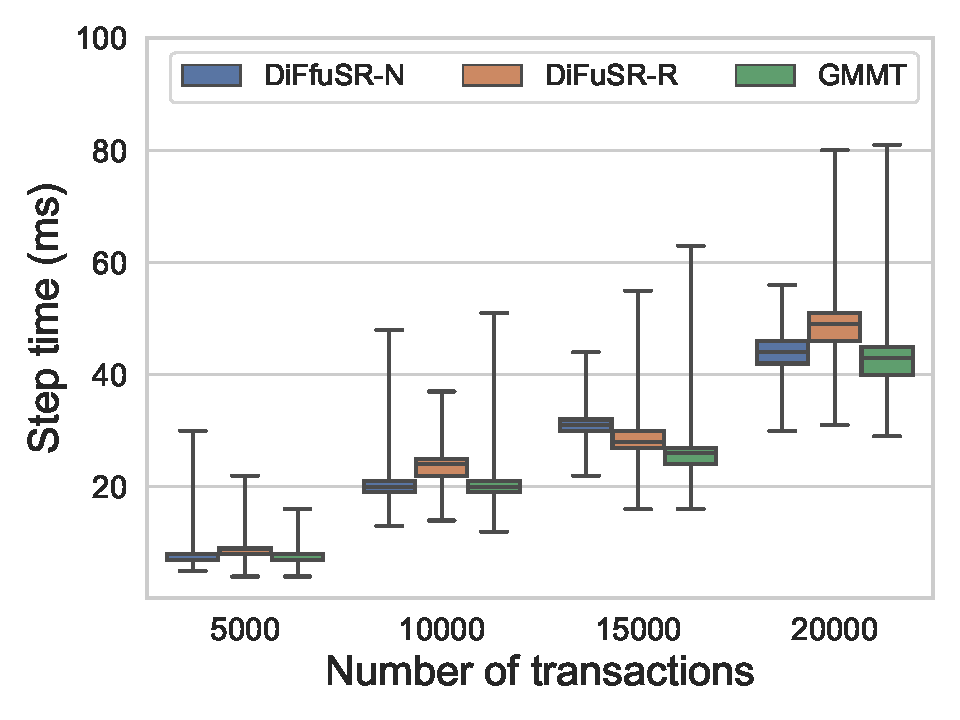
\includegraphics[width=0.5\textwidth]{scalability.pdf} % chktex 8
  \caption{Scalability results: The step time distribution (in milliseconds)
    over 10,000 swaps for increasing values of $\protect\card{\odataset}$. The
    line in each box corresponds to the median, the bottom and top of each box
    correspond to the first and third quartiles, and the lower and upper
    whiskers correspond to the minimum and maximum.}\label{fig:scalability}
\end{figure}%

\begin{figure*}[tb]
  \centering
  \begin{subfigure}{0.33\textwidth}
    \centering
    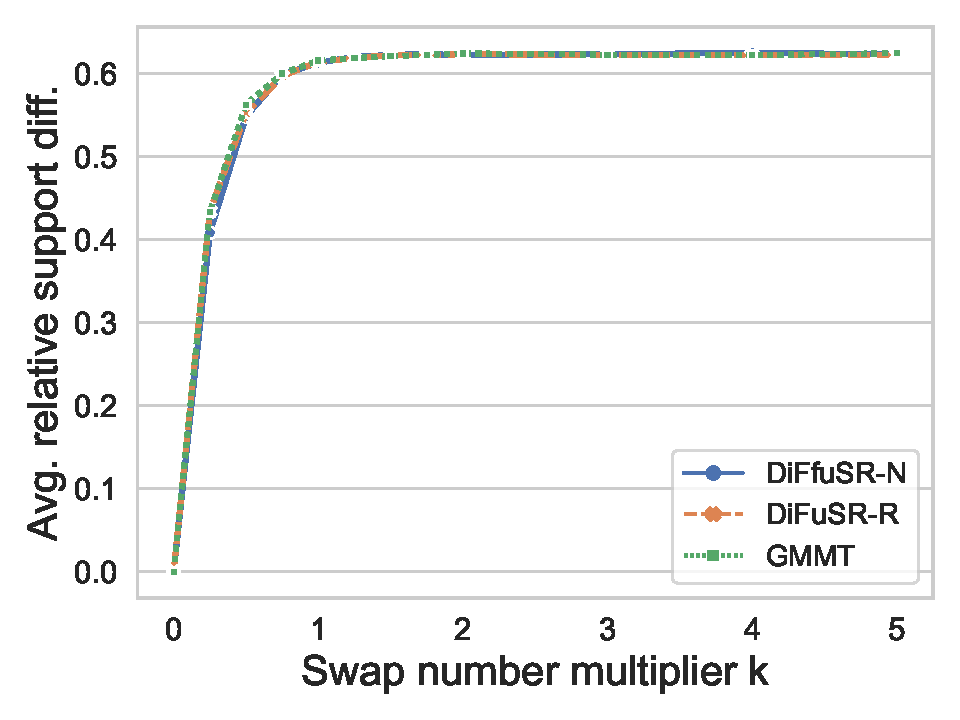
\includegraphics[width=\textwidth]{convergence-foodmart-5-0.0003-0.pdf} % chktex 8
    \caption{\textsc{Foodmart}}
  \end{subfigure}%
  \begin{subfigure}{0.33\textwidth}
    \centering
    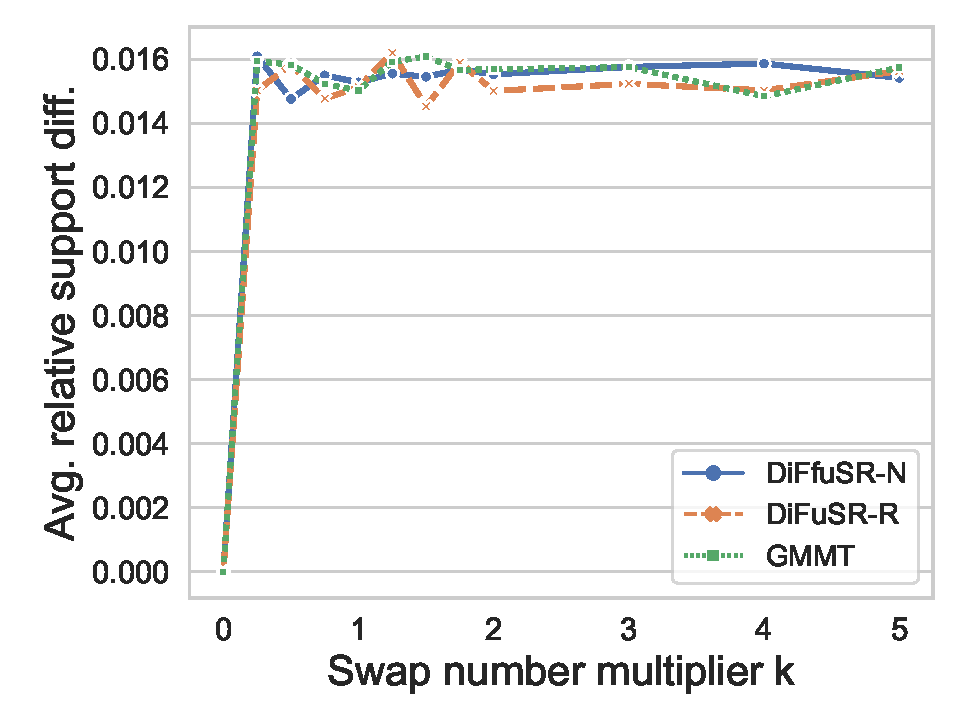
\includegraphics[width=\textwidth]{convergence-chess-5-0.8-0.pdf} % chktex 8
    \caption{\textsc{Chess}}\label{fig:arsdchess}
  \end{subfigure}%
  \begin{subfigure}{0.33\textwidth}
    \centering
    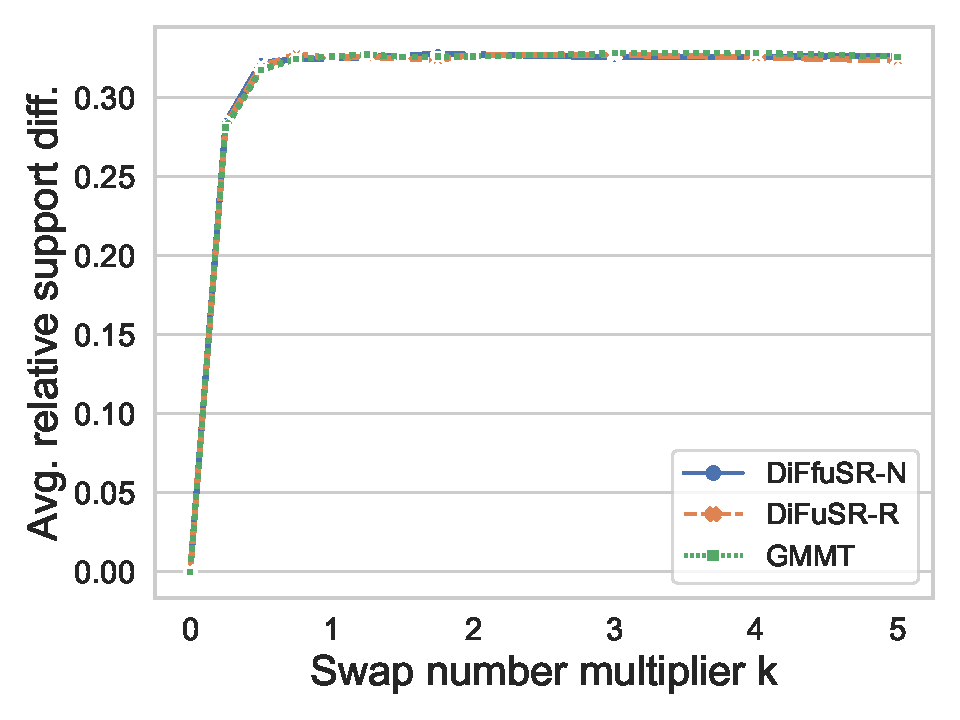
\includegraphics[width=\textwidth]{convergence-mushrooms-5-0.3-0.pdf} % chktex 8
    \caption{\textsc{Mushroom}}
  \end{subfigure}

  \begin{subfigure}{0.33\textwidth}
    \centering
    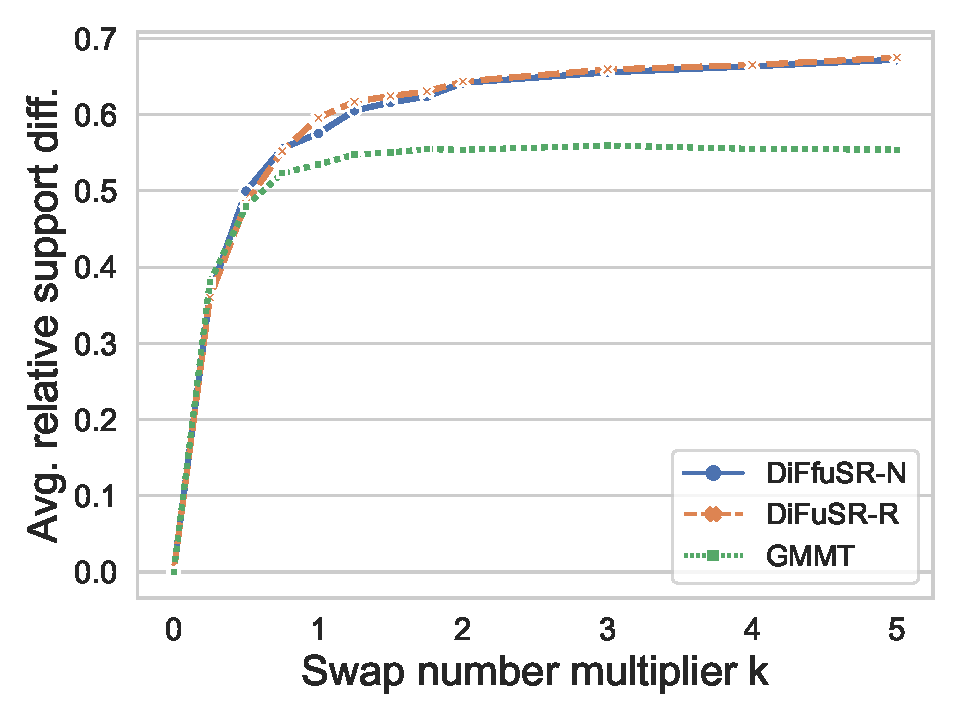
\includegraphics[width=\textwidth]{convergence-BMS1-5-0.001-0.pdf} % chktex 8
    \caption{\textsc{BMS 1}}
  \end{subfigure}%
  \begin{subfigure}{0.33\textwidth}
    \centering
    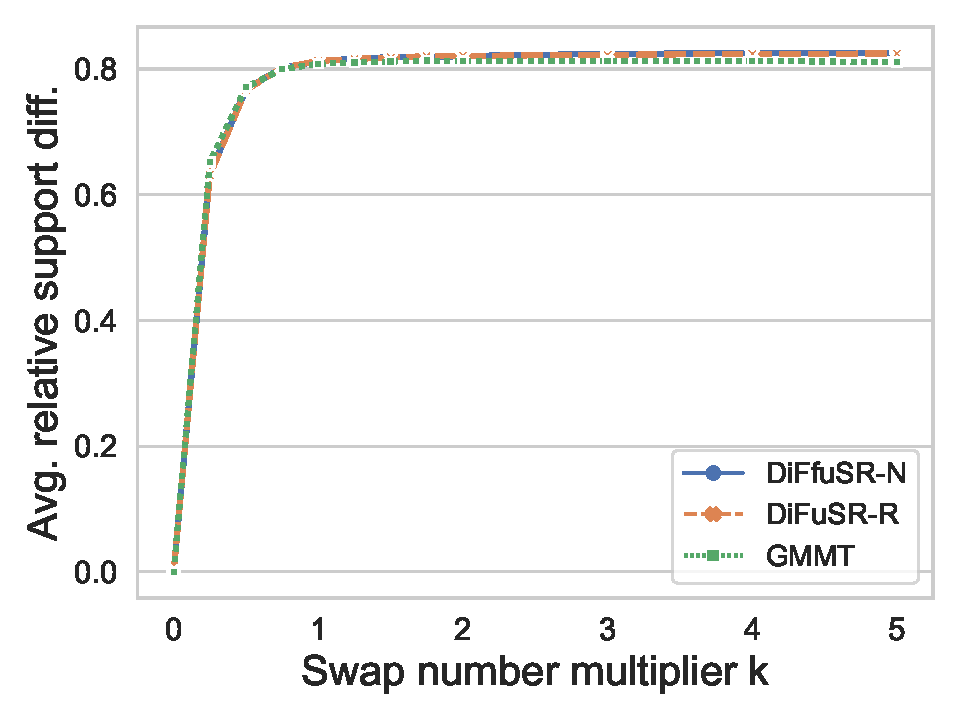
\includegraphics[width=\textwidth]{convergence-BMS2-5-0.002-0.pdf} % chktex 8
    \caption{\textsc{BMS 2}}
  \end{subfigure}
  \caption{Convergence results: $\arsd{\odataset}$ as the swap number multiplier
    $\swapnummult$ grows, where $\swapnummult$ is s.t.\ the number of swaps is
    $\swapnum \doteq \lfloor \swapnummult \sum_{i=1}^m
  \protect\card{t_i}\rfloor$.}\label{fig:arsd}
\end{figure*}

\section{Scalability}

We use the IBM Quest generator to create synthetic datasets with
$\card{\odataset} \in \{$5,000, 10,000, 15,000, 20,000$\}$, on
$\card{\items}=100$ and average transaction length $\card{t}=25$. We run all
algorithms for 10,000 swaps on each dataset, and report the results in
\cref{fig:scalability}.

There is a linear relationship between the distribution of step times and the
number of transactions, as all algorithms need to compute
$\totspairsnummat{M_{\dataset''}}$, which takes time linear in
$\card{\dataset''}$. The interquartile range ($Q3 - Q1$) grows in absolute
terms because the individual step times grow, but it is essentially constant in
relative terms.

\section{Convergence to the Stationary Distribution}

Since we cannot prove an upper bound to the mixing time of the Markov chains
used by our algorithms (see \cref{sec:extensions}), we empirically estimate it.
Following other works using MCMC with MH for swap
randomization~\citep{TononV19}, we estimate the mixing time by tracking the
\emph{Average Relative Support Difference (ARSD)}, defined as follows. Given the
observed dataset $\odataset$, let $\thresh \in \lparen0,\card{\odataset}\rbrack$
be a minimum support threshold, and $\dataset_\swapnum$ be the dataset
corresponding to the state of the chain after $\swapnum \in \mathbb{N}$ swaps.
Then, the average relative support difference $\arsd{\dataset_\swapnum}$ of
$\dataset_\swapnum$ is
\[
  \arsd{\dataset_\swapnum} \doteq \frac{1}{\card{\fis{\thresh}{\odataset}}}
  \sum_{A \in \fis{\thresh}{\odataset}} \frac{\abs{\supp{A}{\odataset} -
  \supp{A}{\dataset_\swapnum}}}{\vphantom{\supp{A}{\nonsmashedodataset}}\supp{A}{\odataset}} \enspace.
  % vphantom for pretty printing
\]
For each dataset, we report $\arsd{\dataset_\swapnum}$ for $\swapnum \doteq
\lfloor \swapnummult \sumtlen \rfloor$ swaps, where $\swapnummult \in \{0, 0.25,
0.50, \dotsc, 2, 3, 4, 5\}$ and $\sumtlen \doteq \sum_{i = 1}^{m} \card{t_i}$,
in \cref{fig:arsd}. We use the values of $\thresh$ from \cref{tab:datasets}:
the qualitative results do not change with other values.

We remark that comparing the mixing times of Markov chains with different
stationary distributions (as \gioalgo\ and \naivealgo) and even on different
sets of states (as \refalgo\ vs.\ the other two) is \emph{meaningless}, as they
allow to sample different objects from different sets according to different
distributions. Neither are the values of the ARSD comparable, as they are
\emph{proxies} for the mixing times, but not for the distance between the state
distribution and the stationary distribution, and they also depend on the chosen
$\thresh$. Therefore, we do not make such comparisons and only include the
results from \gioalgo\ for completeness (the mixing time for
\gioalgo\ is the same observed by \citet[Sect.\ 5.1]{GionisMMT07}).

\Cref{fig:arsd} shows that in all cases, the ARSD stabilizes by $\swapnum = 2
\sumtlen$ swaps or earlier (by $\swapnum = \sumtlen$), i.e., the mixing time
appears to be linear in $\sumtlen$. For \textsc{Chess}, the fluctuations in the
ARSD may seem large due to the scale of the y-axis, which is much smaller in
\cref{fig:arsdchess} than in the other subfigures.

%! TEX root = diffusr.tex
\section{Conclusion}\label{sec:concl}

We present \algo, a collection of algorithms for sampling unlabeled
transactional datasets from a null model, which is a key step in evaluating the
statistical validity of the results of knowledge discovery tasks. \algo\ uses
swap-randomization, a Markov-Chain-Monte-Carlo approach. In contrast with
previous work, \algo\ does not suffer from a distortion of the space of
datasets, which was due to an assumed 1-to-1 mapping of the datasets to binary
matrices. This distortion may (and does) affect the outcome of the validation,
i.e., results in false discoveries. We avoid this assumption and show two
methods (\naivealgo\ and \refalgo) for drawing datasets from the non-distorted
null space. Our experimental evaluation shows that the distortion is relevant,
but \algo\ does not suffer from it, is fast, and scales well as the dataset
grows.

Interesting directions for future work include the definition of richer null
models that capture more important properties of the data, and fast algorithms
to sample from these null models.


%\bibliographystyle{ACM-Reference-Format}
%\bibliography{statseqpat.bib}
%! TEX root = diffusr.tex

\begin{thebibliography}{37}

%%% ====================================================================
%%% NOTE TO THE USER: you can override these defaults by providing
%%% customized versions of any of these macros before the \bibliography
%%% command.  Each of them MUST provide its own final punctuation,
%%% except for \shownote{}, \showDOI{}, and \showURL{}.  The latter two
%%% do not use final punctuation, in order to avoid confusing it with
%%% the Web address.
%%%
%%% To suppress output of a particular field, define its macro to expand
%%% to an empty string, or better, \unskip, like this:
%%%
%%% \newcommand{\showDOI}[1]{\unskip}   % LaTeX syntax
%%%
%%% \def \showDOI #1{\unskip}           % plain TeX syntax
%%%
%%% ====================================================================

\ifx\showCODEN\undefined\def\showCODEN#1{\unskip}\fi
\ifx\showDOI\undefined\def\showDOI#1{#1}\fi
\ifx\showISBNx\undefined\def\showISBNx#1{\unskip}\fi
\ifx\showISBNxiii\undefined\def\showISBNxiii#1{\unskip}\fi
\ifx\showISSN\undefined\def\showISSN#1{\unskip}\fi
\ifx\showLCCN\undefined\def\showLCCN#1{\unskip}\fi
\ifx\shownote\undefined\def\shownote#1{#1}\fi
\ifx\showarticletitle\undefined\def\showarticletitle#1{#1}\fi
\ifx\showURL\undefined\def\showURL{\relax}\fi
% The following commands are used for tagged output and should be
% invisible to TeX
\providecommand\bibfield[2]{#2}
\providecommand\bibinfo[2]{#2}
\providecommand\natexlab[1]{#1}
\providecommand\showeprint[2][]{arXiv:#2}

\bibitem[Agrawal and Srikant(1994)]%
        {AgrawalS94}
\bibfield{author}{\bibinfo{person}{R. Agrawal} {and}
  \bibinfo{person}{R. Srikant}.} \bibinfo{year}{1994}\natexlab{}.
\newblock\showarticletitle{Fast Algorithms for Mining Association Rules in
  Large Databases}. In VLDB'94.

\bibitem[Bonferroni(1936)]%
        {Bonferroni37}
\bibfield{author}{\bibinfo{person}{C.\ E. Bonferroni}.}
  \bibinfo{year}{1936}\natexlab{}.
\newblock\showarticletitle{Teoria statistica delle classi e calcolo delle
  probabilit{\`a}}.
\newblock\bibinfo{journal}{\emph{Pubb.\ R.\ Inst.\ Sup.\ Sci.\ Econ. Commerc.\
Firenze}}  \bibinfo{volume}{8} (\bibinfo{year}{1936}), \bibinfo{pages}{3--62}.

\bibitem[Brin et~al\mbox{.}(1997)]%
        {BrinMS97}
\bibfield{author}{\bibinfo{person}{S. Brin}, \bibinfo{person}{R.
  Motwani}, {and} \bibinfo{person}{C. Silverstein}.}
  \bibinfo{year}{1997}\natexlab{}.
\newblock\showarticletitle{Beyond market baskets: Generalizing association
  rules to correlations}. In SIGMOD'97.

\bibitem[Duivesteijn and Knobbe(2011)]%
        {DuivesteijnK11}
\bibfield{author}{\bibinfo{person}{W. Duivesteijn} {and}
  \bibinfo{person}{A. Knobbe}.} \bibinfo{year}{2011}\natexlab{}.
\newblock\showarticletitle{Exploiting False Discoveries --- Statistical
  Validation of Patterns and Quality Measures in Subgroup Discovery}. In
  ICDM'11.

\bibitem[Ferkingstad et~al\mbox{.}(2015)]%
        {FerkingstadHS15}
\bibfield{author}{\bibinfo{person}{E. Ferkingstad}, \bibinfo{person}{L. Holden},
  {and} \bibinfo{person}{G. K. Sandve}.}
  \bibinfo{year}{2015}\natexlab{}.
\newblock\showarticletitle{{Monte Carlo} Null Models for Genomic Data}.
\newblock\bibinfo{journal}{\emph{Statist. Sci.}} \bibinfo{volume}{30},
  \bibinfo{number}{1} (\bibinfo{year}{2015}), \bibinfo{pages}{59--71}.

\bibitem[Gionis et~al\mbox{.}(2007)]%
        {GionisMMT07}
\bibfield{author}{\bibinfo{person}{A. Gionis}, \bibinfo{person}{H. Mannila},
  \bibinfo{person}{T. Mielik{\"a}inen}, {and} \bibinfo{person}{P. Tsaparas}.}
  \bibinfo{year}{2007}\natexlab{}.
\newblock\showarticletitle{Assessing data mining results via swap
  randomization}.
\newblock\bibinfo{journal}{\emph{ACM TKDD}} \bibinfo{volume}{1}, \bibinfo{number}{3}
  (\bibinfo{year}{2007}), \bibinfo{pages}{14}.

\bibitem[G{\"u}nnemann et~al\mbox{.}(2012)]%
        {GunnemannDJE12}
\bibfield{author}{\bibinfo{person}{S. G{\"u}nnemann},
  \bibinfo{person}{P. Dao}, \bibinfo{person}{M. Jamali}, {and}
  \bibinfo{person}{M. Ester}.} \bibinfo{year}{2012}\natexlab{}.
\newblock\showarticletitle{Assessing the Significance of Data Mining Results
  on Graphs with Feature Vectors}. In ICDM'12.

\bibitem[H{\"a}m{\"a}l{\"a}inen(2010)]%
        {Hamalainen10}
\bibfield{author}{\bibinfo{person}{W. H{\"a}m{\"a}l{\"a}inen}.}
  \bibinfo{year}{2010}\natexlab{}.
\newblock\showarticletitle{{StatApriori}: an efficient algorithm for searching
  statistically significant association rules}.
\newblock\bibinfo{journal}{\emph{KAIS}}
  \bibinfo{volume}{23}, \bibinfo{number}{3} (\bibinfo{year}{2010}),
  \bibinfo{pages}{373--399}.

\bibitem[H{\"a}m{\"a}l{\"a}inen and Webb(2019)]%
        {HamalainenW19}
\bibfield{author}{\bibinfo{person}{W. H{\"a}m{\"a}l{\"a}inen} {and}
  \bibinfo{person}{G.\ I. Webb}.} \bibinfo{year}{2019}\natexlab{}.
\newblock\showarticletitle{A tutorial on statistically sound pattern
  discovery}.
\newblock\bibinfo{journal}{\emph{DMKD}}
  \bibinfo{volume}{33}, \bibinfo{number}{2} (\bibinfo{year}{2019}),
  \bibinfo{pages}{325--377}.

\bibitem[Hanhij{\"a}rvi(2011)]%
        {Hanhijarvi11}
\bibfield{author}{\bibinfo{person}{S. Hanhij{\"a}rvi}.}
  \bibinfo{year}{2011}\natexlab{}.
\newblock\showarticletitle{Multiple hypothesis testing in pattern discovery}.
  In DS'11.

\bibitem[Hanhij{\"a}rvi et~al\mbox{.}(2009)]%
        {HanhijarviGP09}
\bibfield{author}{\bibinfo{person}{S. Hanhij{\"a}rvi},
  \bibinfo{person}{G.\ C. Garriga}, {and} \bibinfo{person}{K. Puolam{\"a}ki}.}
  \bibinfo{year}{2009}\natexlab{}.
\newblock\showarticletitle{Randomization Techniques for Graphs}. In SDM'09.


\bibitem[Hanhij\"{a}rvi et~al\mbox{.}(2009)]%
        {HanhijarviOVPTM09}
\bibfield{author}{\bibinfo{person}{S. Hanhij\"{a}rvi},
  \bibinfo{person}{M. Ojala}, \bibinfo{person}{N. Vuokko},
  \bibinfo{person}{K. Puolam\"{a}ki}, \bibinfo{person}{N. Tatti}, {and}
  \bibinfo{person}{H. Mannila}.} \bibinfo{year}{2009}\natexlab{}.
\newblock\showarticletitle{Tell Me Something {I} Don't Know: Randomization
  Strategies for Iterative Data Mining}. In KDD'09.

\bibitem[Holm(1979)]%
        {Holm79}
\bibfield{author}{\bibinfo{person}{S. Holm}.}
  \bibinfo{year}{1979}\natexlab{}.
\newblock\showarticletitle{A simple sequentially rejective multiple test
  procedure}.
\newblock\bibinfo{journal}{\emph{Scand.\ J. Stat.}}
  \bibinfo{volume}{6}, \bibinfo{number}{2} (\bibinfo{year}{1979}),
  \bibinfo{pages}{65--70}.

\bibitem[Kirsch et~al\mbox{.}(2012)]%
        {KirschMPPUV12}
\bibfield{author}{\bibinfo{person}{A. Kirsch}, \bibinfo{person}{M.
  Mitzenmacher}, \bibinfo{person}{A. Pietracaprina},
  \bibinfo{person}{G. Pucci}, \bibinfo{person}{E. Upfal}, {and}
  \bibinfo{person}{F. Vandin}.} \bibinfo{year}{2012}\natexlab{}.
\newblock\showarticletitle{An efficient rigorous approach for identifying
  statistically significant frequent itemsets}.
\newblock\bibinfo{journal}{\emph{JACM}}
  \bibinfo{volume}{59}, \bibinfo{number}{3} (\bibinfo{year}{2012}),
  \bibinfo{pages}{1--22}.

\bibitem[Komiyama et~al\mbox{.}(2017)]%
        {KomiyamaIANM17}
\bibfield{author}{\bibinfo{person}{J. Komiyama}, \bibinfo{person}{M.
  Ishihata}, \bibinfo{person}{H. Arimura}, \bibinfo{person}{T.
  Nishibayashi}, {and} \bibinfo{person}{S.-I. Minato}.}
  \bibinfo{year}{2017}\natexlab{}.
\newblock\showarticletitle{Statistical Emerging Pattern Mining with Multiple
  Testing Correction}. In KDD'17.

\bibitem[Kontonasios et~al\mbox{.}(2012)]%
        {KontonasiosSDB12}
\bibfield{author}{\bibinfo{person}{K.-N. Kontonasios},
  \bibinfo{person}{E. Spyropoulou}, {and} \bibinfo{person}{T. De~Bie}.}
  \bibinfo{year}{2012}\natexlab{}.
\newblock\showarticletitle{Knowledge discovery interestingness measures based
  on unexpectedness}.
\newblock\bibinfo{journal}{\emph{{WIREs} DMKD}}
  \bibinfo{volume}{2}, \bibinfo{number}{5} (\bibinfo{year}{2012}),
  \bibinfo{pages}{386--399}.

\bibitem[Megiddo and Srikant(1998)]%
        {MegiddoS98}
\bibfield{author}{\bibinfo{person}{N. Megiddo} {and}
  \bibinfo{person}{R. Srikant}.} \bibinfo{year}{1998}\natexlab{}.
\newblock\showarticletitle{Discovering predictive association rules}. In
KDD'94.

\bibitem[Llinares-L{\'o}pez et~al\mbox{.}(2015)]%
        {LlinaresLopezSPB15}
\bibfield{author}{\bibinfo{person}{F. Llinares-L{\'o}pez},
  \bibinfo{person}{M.Sugiyama}, \bibinfo{person}{L. Papaxanthos},
  {and} \bibinfo{person}{K. Borgwardt}.} \bibinfo{year}{2015}\natexlab{}.
\newblock\showarticletitle{Fast and memory-efficient significant pattern
  mining via permutation testing}. In KDD'15.

\bibitem[Low-Kam et~al\mbox{.}(2013)]%
        {LowKRKP13}
\bibfield{author}{\bibinfo{person}{C. Low-Kam}, \bibinfo{person}{C.
  Ra{\"\i}ssi}, \bibinfo{person}{M. Kaytoue}, {and} \bibinfo{person}{J.
  Pei}.} \bibinfo{year}{2013}\natexlab{}.
\newblock\showarticletitle{Mining statistically significant sequential
  patterns}. In ICDM'13.

\bibitem[Minato et~al\mbox{.}(2014)]%
        {MinatoUTTS14}
\bibfield{author}{\bibinfo{person}{S.-I. Minato}, \bibinfo{person}{T.
  Uno}, \bibinfo{person}{K. Tsuda}, \bibinfo{person}{A. Terada}, {and}
  \bibinfo{person}{J. Sese}.} \bibinfo{year}{2014}\natexlab{}.
\newblock\showarticletitle{A fast method of statistical assessment for
  combinatorial hypotheses based on frequent itemset enumeration}. In
  ECML'PKDD'14.

\bibitem[Mitzenmacher and Upfal(2005)]%
        {MitzenmacherU05}
\bibfield{author}{\bibinfo{person}{M. Mitzenmacher} {and}
  \bibinfo{person}{E. Upfal}.} \bibinfo{year}{2005}\natexlab{}.
\newblock\bibinfo{booktitle}{\emph{Probability and Computing: Randomized
  Algorithms and Probabilistic Analysis}}.
\newblock\bibinfo{publisher}{Cambridge University Press}.

\bibitem[Ojala(2010)]%
        {Ojala10}
\bibfield{author}{\bibinfo{person}{M. Ojala}.}
  \bibinfo{year}{2010}\natexlab{}.
\newblock\showarticletitle{Assessing Data Mining Results on Matrices with
  Randomization}. In ICDM'10.

\bibitem[Ojala et~al\mbox{.}(2010)]%
        {OjalaGGM10}
\bibfield{author}{\bibinfo{person}{M. Ojala}, \bibinfo{person}{G.\ C.
  Garriga}, \bibinfo{person}{A. Gionis}, {and} \bibinfo{person}{H.
  Mannila}.} \bibinfo{year}{2010}\natexlab{}.
\newblock\showarticletitle{Evaluating Query Result Significance in Databases
  via Randomizations}. In SDM'10.

\bibitem[Ojala et~al\mbox{.}(2008)]%
        {OjalaVKHM08}
\bibfield{author}{\bibinfo{person}{M. Ojala}, \bibinfo{person}{N.
  Vuokko}, \bibinfo{person}{A. Kallio}, \bibinfo{person}{N. Haiminen},
  {and} \bibinfo{person}{H. Mannila}.} \bibinfo{year}{2008}\natexlab{}.
\newblock\showarticletitle{Randomization of real-valued matrices for assessing
  the significance of data mining results}. In SDM'08.

\bibitem[Pellegrina et~al\mbox{.}(2019a)]%
        {PellegrinaRV19b}
\bibfield{author}{\bibinfo{person}{L. Pellegrina},
  \bibinfo{person}{M. Riondato}, {and} \bibinfo{person}{F. Vandin}.}
  \bibinfo{year}{2019}\natexlab{a}.
\newblock\showarticletitle{Hypothesis Testing and Statistically-sound Pattern
  Mining}. In KDD'19.

\bibitem[Pellegrina et~al\mbox{.}(2019b)]%
        {PellegrinaRV19a}
\bibfield{author}{\bibinfo{person}{L. Pellegrina},
  \bibinfo{person}{M. Riondato}, {and} \bibinfo{person}{F. Vandin}.}
  \bibinfo{year}{2019}\natexlab{b}.
\newblock\showarticletitle{{SPuManTE}: Significant Pattern Mining with
  Unconditional Testing}. In KDD'19.

\bibitem[Pellegrina and Vandin(2020)]%
        {PellegrinaV20}
\bibfield{author}{\bibinfo{person}{L. Pellegrina} {and}
  \bibinfo{person}{F. Vandin}.} \bibinfo{year}{2020}\natexlab{}.
\newblock\showarticletitle{Efficient mining of the most significant patterns
  with permutation testing}.
\newblock\bibinfo{journal}{\emph{DMKD}}
  \bibinfo{volume}{34} (\bibinfo{year}{2020}), \bibinfo{pages}{1201--1234}.

\bibitem[Stanley(2011)]%
        {Stanley11}
\bibfield{author}{\bibinfo{person}{R.~P. Stanley}.}
  \bibinfo{year}{2011}\natexlab{}.
\newblock\bibinfo{booktitle}{\emph{Enumerative Combinatorics}
  (\bibinfo{edition}{2} ed.)}. Vol.~\bibinfo{volume}{1}.
\newblock\bibinfo{publisher}{Cambridge University Press}.

\bibitem[Tan et~al\mbox{.}(2004)]%
        {TanKS04}
\bibfield{author}{\bibinfo{person}{P.-N. Tan}, \bibinfo{person}{V.
  Kumar}, {and} \bibinfo{person}{J. Srivastava}.}
  \bibinfo{year}{2004}\natexlab{}.
\newblock\showarticletitle{Selecting the right objective measure for
  association analysis}.
\newblock\bibinfo{journal}{\emph{Inf. Sys.}}  \bibinfo{volume}{29}
  (\bibinfo{year}{2004}), \bibinfo{pages}{293--313}.

\bibitem[Terada et~al\mbox{.}(2013)]%
        {TeradaOHTS13}
\bibfield{author}{\bibinfo{person}{A. Terada}, \bibinfo{person}{M.
  Okada-Hatakeyama}, \bibinfo{person}{K. Tsuda}, {and} \bibinfo{person}{J.
  Sese}.} \bibinfo{year}{2013}\natexlab{}.
\newblock\showarticletitle{Statistical significance of combinatorial
  regulations}.
\newblock\bibinfo{journal}{\emph{PNAS}} \bibinfo{volume}{110}, \bibinfo{number}{32}
  (\bibinfo{year}{2013}), \bibinfo{pages}{12996--13001}.

\bibitem[Tonon and Vandin(2019)]%
        {TononV19}
\bibfield{author}{\bibinfo{person}{A. Tonon} {and} \bibinfo{person}{F.
  Vandin}.} \bibinfo{year}{2019}\natexlab{}.
\newblock\showarticletitle{Permutation strategies for mining significant
  sequential patterns}. In ICDM'19.

\bibitem[Vreeken and Tatti(2014)]%
        {VreekenT14}
\bibfield{author}{\bibinfo{person}{J. Vreeken} {and}
  \bibinfo{person}{N. Tatti}.} \bibinfo{year}{2014}\natexlab{}.
\newblock\showarticletitle{Interesting patterns}.
\newblock%
In \bibinfo{booktitle}{\emph{Frequent pattern mining}}.
  \bibinfo{publisher}{Springer}, \bibinfo{pages}{105--134}.

\bibitem[Wasserman(2005)]%
        {Wasserman05}
\bibfield{author}{\bibinfo{person}{L. Wasserman}.}
  \bibinfo{year}{2005}\natexlab{}.
\newblock\bibinfo{booktitle}{\emph{All of Statistics: A Concise Course in
  Statistical Inference}}.
\newblock\bibinfo{publisher}{Springer}.

\bibitem[Webb(2006)]%
        {Webb06}
\bibfield{author}{\bibinfo{person}{G.\ I. Webb}.}
  \bibinfo{year}{2006}\natexlab{}.
\newblock\showarticletitle{Discovering significant rules}. In KDD'06.

\bibitem[Webb(2007)]%
        {Webb07}
\bibfield{author}{\bibinfo{person}{G.\ I. Webb}.}
  \bibinfo{year}{2007}\natexlab{}.
\newblock\showarticletitle{Discovering significant patterns}.
\newblock\bibinfo{journal}{\emph{Mach.\ Learn.}} \bibinfo{volume}{68},
  \bibinfo{number}{1} (\bibinfo{year}{2007}), \bibinfo{pages}{1--33}.

\bibitem[Webb(2008)]%
        {Webb08}
\bibfield{author}{\bibinfo{person}{G.\ I Webb}.}
  \bibinfo{year}{2008}\natexlab{}.
\newblock\showarticletitle{Layered critical values: a powerful
  direct-adjustment approach to discovering significant patterns}.
\newblock\bibinfo{journal}{\emph{Mach.\ Learn.}} \bibinfo{volume}{71},
  \bibinfo{number}{2--3} (\bibinfo{year}{2008}), \bibinfo{pages}{307--323}.

\bibitem[Westfall and Young(1993)]%
        {WestfallY93}
\bibfield{author}{\bibinfo{person}{P.\ H. Westfall} {and}
  \bibinfo{person}{S.\ S. Young}.} \bibinfo{year}{1993}\natexlab{}.
\newblock\bibinfo{booktitle}{\emph{Resampling-Based Multiple Testing: Examples
  and Methods for {p}-Value Adjustment}}.
\newblock\bibinfo{publisher}{Wiley-Interscience}.

\bibitem[Wu et~al\mbox{.}(2016)]%
        {WuHGLZY16}
\bibfield{author}{\bibinfo{person}{J. Wu}, \bibinfo{person}{Z. He},
  \bibinfo{person}{F. Gu}, \bibinfo{person}{X. Liu},
  \bibinfo{person}{J. Zhou}, {and} \bibinfo{person}{C. Yang}.}
  \bibinfo{year}{2016}\natexlab{}.
\newblock\showarticletitle{Computing exact permutation {$p$}-values for
  association rules}.
\newblock\bibinfo{journal}{\emph{Inf.\ Sci.}}  \bibinfo{volume}{346}
  (\bibinfo{year}{2016}), \bibinfo{pages}{146--162}.

\end{thebibliography}


\clearpage % new page in two-columns layout
\appendix
%! TEX root = diffusr.tex

\section{Appendix}\label{sec:appendix}

\subsection{Missing Proofs}\label{sec:missingproofs}

\begin{proof}[Proof of \cref{lem:wrongsampling}]
  Let $\odataset = \{ \{1, 2\}, \{1, 3\}, \{3\} \}$, and assume, w.l.o.g., that
  $\odataset'$ is the seq-dataset $\dataset'$ from~\eqref{eq:sampledataset},
  then clearly the matrix $M_{\dataset'}$ from~\eqref{eq:sampledatasetmatrix}
  belongs to $\matrices$.

  The set $\matrices$ also contains the matrix $M''$ obtained by swapping the
  first two rows of $M_{\dataset'}$ from~\eqref{eq:sampledatasetmatrix}, which
  corresponds to the seq-dataset $\dataset'' = \langle \{1, 3\}, \{1, 2\}, \{3\}
  \rangle$. The seq-datasets $\dataset'$ from~\eqref{eq:sampledataset} and
  $\dataset''$ are \emph{different}, but their corresponding datasets
  respectively are \emph{the same dataset}, i.e., $\mattodat{M_{\dataset'}} =
  \mattodat{M''}$. Thus, the set $\matrices$ contains \emph{at least two}
  matrices mapped to seq-datasets that, when seen as bags, are equal to
  $\odataset$. From the definition of $\matrices$, it holds that $\matrices$
  also contains
  \[
    A \doteq \left[
    \begin{array}{ccc}
      1 & 0 & 1 \\
      1 & 0 & 1 \\
      0 & 1 & 0
    \end{array}
    \right] \enspace.
  \]
  It holds that $\mattodat{A} = \{\{1,3\}, \{1, 3\}, \{2\}\}$. Again from the
  definition of $\matrices$, it holds that there is no other matrix $B$
  different than $A$ in $\matrices$ such that $\mattodat{B}= \mattodat{A}$.
  Thus, if we sample a matrix $M$ uniformly at random from $\matrices$ there is
  a higher probability that $\mattodat{M} = \odataset$ than $\mattodat{M} =
  \mattodat{A}$, and our proof is complete.
\end{proof}

\begin{proof}[Proof of \cref{lem:numcopies}]
  Recall that $\matrices$ depends on the observed dataset $\odataset$ and on the
  arbitrary ordering of its transactions chosen by \gioalgo, as the ordering
  fixes the row-sums $\rowsum{i}$, $1 \le i \le \rowsnum$ of the matrices in
  $\matrices$. In other words, it fixes the row indices of rows corresponding to
  transactions of length $\ell_i$, $1 \le i \le z_\dataset$, of
  $\dataset$. Thus, the number of different ways in which the transactions of
  $\dataset$ can be assigned to the rows of a matrix in $\matrices$ is the
  product, over the lengths in $L_\dataset$, of the number $q_i$ of different
  ways in which the transactions in $T_i$ can be assigned, i.e.,
  \[
    \copiesnum{\dataset} = \prod_{i=1}^{z_\dataset} q_i \enspace.
  \]
  Thus, we only have to argue that
  \[
    q_i = \binom{\card{T_i}}{\card{W_{i,1}}, \dotsc,
    \card{W_{i,h_i}}},
  \]
  which is true because the multinomial coefficient $\binom{n}{k_1,\dotsc,k_h}$
  is the number of different permutations of a bag containing $n$ objects such
  that $k_1$ objects are indistinguishable among themselves and of type 1, $k_2$
  objects are indistinguishable among themselves and of type 2, and so
  on~\citep[Eq.~1.22]{Stanley11}.
\end{proof}

\begin{proof}[Proof of \cref{thm:correctnaive}]
 A dataset $\dataset  \in \nullset$ is returned in output by \naivealgo\ iff a
 matrix $M$ such that $\mattodat{M} = \dataset$ is sampled. There are
 $\copiesnum{\dataset}$ such matrices $M$, each with a probability
 $\samplprob(M)$ as in~\eqref{eq:naivestatprob} to be sampled, from the
 properties of MCMC sampling with MH\@. Thus, the probability of returning
 $\dataset$ is exactly $\nullprob(\dataset$).
\end{proof}

\begin{proof}[Proof of \cref{lem:spairsnum}]
  We start by showing that, independently from the value of
  $\spairsfactor(t_a,t_b)$, all the swaps from $\dataset'$ to $\dataset''$ must
  involve transactions that are identical to $t_a$ and $t_b$, i.e, be in the
  form $((t_a,x),(t_b,y))$, for some $x,y\in \items$. Let $((t_c,c), (t_d,d))$
  be a swap from $\dataset'$ to $\dataset''$. We want to show that $((t_c,c),
  (t_d,d)) = ((t_a,a),(t_b,b))$.  Let $\bar{t}_a = (t_a \setminus \{a\}) \cup
  \{b\}$, $\bar{t}_b = (t_b \setminus \{b\}) \cup \{a\}$, $\bar{t}_c = (t_c
  \setminus \{c\}) \cup \{d\}$, and $\bar{t}_d = (t_d \setminus \{d\}) \cup
  \{c\}$. Then,
  \[
    (\dataset' \setminus \{ t_a, t_b \}) \cup \{ \bar{t}_a, \bar{t}_b \} =
    (\dataset' \setminus \{ t_c, t_d \}) \cup \{ \bar{t}_c, \bar{t}_d \}
  \]
  since both sides are equal to $\dataset''$. Since datasets are \emph{bags}, the
  operations of difference and union are effectively one the inverse of the
  other. Thus, we can write
  \[
    \dataset' \cup \{ \bar{t}_a, \bar{t}_b \} \cup \{ t_c, t_d \} = \dataset'
    \cup \{ \bar{t}_c, \bar{t}_d \} \cup \{ t_a, t_b \} \enspace.
  \]
  We can remove $\dataset'$ from both sides to get
  \begin{equation}\label{eq:spairsnumtech}
    \{ \bar{t}_a, \bar{t}_b, t_c, t_d \} = \{ \bar{t}_c, \bar{t}_d, t_a, t_b \}
    \enspace.
  \end{equation}
  By definition of a swap, it must be $t_a \neq \bar{t}_a$ and $t_a \neq
  \bar{t}_b$, thus it must be either $t_a = t_c$ or $t_a = t_d$, and similarly
  for $t_b$.

  Assume now that $\card{t_a} \neq \card{t_b}$, then only one between $t_a =
  t_c$ and $t_a = t_d$ is actually possible so, w.l.o.g., let $t_a = t_c$ and
  $t_b = t_d$. Then from these facts and~\eqref{eq:spairsnumtech}, it must be
  $\{ \bar{t}_a, \bar{t}_b \} = \{ \bar{t}_c, \bar{t}_d \}$, thus either
  $\bar{t}_a = \bar{t}_c$ or $\bar{t}_a = \bar{t}_d$. Since $\card{\bar{t}_a} =
  \card{t_a} = \card{t_c} = \card{\bar{t}_c}$ and $\card{\bar{t}_d} =
  \card{t_d} = \card{t_b}$, then it can only be $\bar{t}_a = \bar{t}_c$, which
  implies $c = a$, and similarly it must be $b = d$. Thus, if $\card{t_a} \neq
  \card{t_b}$, then all swaps from $\dataset'$ to $\dataset''$ are equal to
  $((t_a,a), (t_b,b))$, which implies the thesis for this case.

  Assume now that $\card{t_a} = \card{t_b}$ but $\card{t_a \setminus t_b}$ and
  $\card{t_b \setminus t_a}$ are different than 2 (the two asymmetric set
  differences must have the same size, since the two sets have the same size).
  From the first part of the proof, we have that it must be either $t_a = t_c$
  or $t_a = t_d$, and similarly for $t_b$. W.l.o.g., let $t_a = t_c$ and $t_b =
  t_d$.  If $\card{t_a \setminus t_b} = \card{t_b \setminus t_a} = 1$, then $a$
  and $b$ are the only two items that can be swapped, so it must be $c = a$ and
  $b = d$. Thus, in this specific subcase, all swaps from $\dataset'$ to
  $\dataset''$ are equal to $((t_a,a), (t_b,b))$, which implies the thesis for
  this case. Assume now that $\card{t_a \setminus t_b} = \card{t_b \setminus
  t_a} > 2$.  From these facts and~\eqref{eq:spairsnumtech}, it must be $\{
  \bar{t}_a, \bar{t}_b \} = \{ \bar{t}_c, \bar{t}_d \}$, thus either $\bar{t}_a
  = \bar{t}_c$ or $\bar{t}_a = \bar{t}_d$. We now show that it must be
  $\bar{t}_a = \bar{t}_c$. Assume by contradiction that $\bar{t}_a = \bar{t}_d$.
  Since $t_c = t_a$, it holds $\bar{t}_a = t_c \setminus \{a\} \cup \{b\}$.
  Thus, it must be
  \[
    (t_c \setminus \{a\}) \cup \{b\} = (t_d \setminus \{d\}) \cup \{c\} \enspace.
  \]
  Since $a, c \in t_c$ and $b \notin t_c$, by taking the asymmetric set
  differences between each side of the above identity and $t_c$ we get
  \[
    \{ b \} = (t_d \setminus \{d \}) \setminus t_c
  \]
  which means that $t_d \setminus t_c  = t_b \setminus t_a = \{b, d\}$, i.e.,
  this set difference has size equal to 2, which is a contradiction since we
  assumed that $\card{t_b \setminus t_a} > 2$. Thus, it must be $\bar{t}_a =
  \bar{t}_c$, which implies $c = a$, and similarly it must be $b = d$. Thus, all
  swaps from $\dataset'$ to $\dataset''$ are equal to $((t_a,a), (t_b,b))$,
  which implies the thesis for this case.

  We have therefore shown that the thesis is true for the case
  $\spairsfactor(t_a,t_b)=1$. Consider now the other case, which means that
  $\card{t_a} = \card{t_b}$ and $\card{t_a \setminus t_b} = \card{t_b \setminus
  t_a} = 2$. W.l.o.g., let $t_a \setminus t_b = \{a, z\}$ and $t_b \setminus t_a
  = \{b, w\}$.  It is easy to see that the swaps $((t_a,a), (t_b,b))$ and
  $((t_a,z), (t_b,w))$ lead to the same dataset $\dataset''$, while the other
  two swaps $((t_a,a), (t_b,w))$ $((t_a,z), (t_b,b))$ lead to a different
  dataset. Thus, there are $\spairsfactor(t_a,t_b)=2$ swaps from $\dataset'$ to
  $\dataset''$ involving the transactions $t_a$ and $t_b$. From the first part
  of the proof, we have that all swaps from $\dataset'$ to $\dataset''$ must
  involve transactions identical to $t_a$ and $t_b$, hence we obtain the thesis
  for this case.
\end{proof}

\begin{proof}[Proof of \cref{thm:totspairsnumdat}]
  Let $((t_a, a), (t_b, b))$ be any of the $\totspairsnummat{M_\dataset}$
  swaps from $M_\dataset$ to any $M$ of its neighbor matrices in the Markov
  chain used by \gioalgo. From the definitions of ``swap'' for \gioalgo\ and for
  \refalgo, it follows that $((t_a, a), (t_b, b))$ is a valid swap for
  $\refalgo$ iff $\mattodat{M} \neq \dataset$, i.e., if the dataset
  corresponding to $M$ is not $\dataset$ itself. The number of valid
  swaps from $\dataset$ is therefore $\totspairsnummat{M_\dataset}$ minus the
  total number of swaps from $M_\dataset$ to any $M$ of its neighbors with
  $\mattodat{M} = \dataset$. We now show that the number of such
  ``self-swaps'' is $\selfspairsnum{\dataset}$.

  For a neighbor $M \neq M_\dataset$ of $M_\dataset$ to have $\mattodat{M} =
  \dataset$ it must be that that there is a swap $((t_a, a), (t_b, b))$ such
  that
  \[
    (t_a \setminus \{a\}) \cup \{b\} = t_b\ \text{and}\ (t_b \setminus \{b\})
    \cup \{a\}=t_a \enspace.
  \]
  Since $a \in t_a \setminus t_b$ and $b \in t_b \setminus t_a$, the above is
  possible iff $\card{t_a} = \card{t_b}$ and $\{a\} = t_a \setminus t_b$ and
  $\{b\} = t_b \setminus t_a$. The number of such \emph{unordered} pairs of
  transactions (i.e., the number of self-swaps) is as
  in~\eqref{eq:selfspairsnum}, where the factor $\sfrac{1}{2}$ is to correct for
  the fact that the considered set contains \emph{ordered} pairs of
  transactions.
\end{proof}

\begin{proof}[Proof of \cref{lem:sampleneighbor}]
  The procedure keeps sampling candidate swaps (i.e., pairs of elements of
  $\spairs$) until it finds one that is a valid swap. Since each element of
  $\spairs$ is sampled independently and uniformly at random from $\spairs$,
  then the candidate swap is chosen uniformly at random among all candidate
  swaps, thus, if it is valid, is also chosen uniformly at random among all
  valid swaps, i.e., each valid swap has a probability of
  $1/\totspairsnumdat{\dataset'}$ of being chosen among all valid swaps, as
  there is one and only one pair of elements of $\spairs$ for each valid swap.
  $\dataset''$ is output whenever the procedure chooses one of the
  $\spairsnum{\dataset'}{\dataset''}$ valid swaps leading to it from
  $\dataset'$. Thus, the probability of outputting $\dataset''$ is the sum of
  the probabilities of choosing each of these swaps, hence the thesis.
\end{proof}

\subsection{Computing $\copiesnum{\mattodat{M''}}$ from
  $\copiesnum{\mattodat{M'}}$}\label{sec:copiesnum}

Using the notation from the statement of \cref{lem:numcopies}, given a
transaction $t \in \mattodat{M'}$, suppose $t \in T_i$ for $1 \leq i \leq
z_{\mattodat{M'}}$. Further suppose $t = \tau_{i, j} \in \bar{T}_i$, where $1
\leq j \leq h_i$. Let $\mathsf{net}$ be a dictionary that maps each different
transaction $t \in \mattodat{M'}$ to $\card{W_{i, j}}$, i.e., the size of the
bag of transactions equal to $t$ (including $t$). This data structure is easy to
initialize and keep up to date. We can then obtain $\copiesnum{\mattodat{M'}}$
from $\copiesnum{\mattodat{M''}}$ as shown in \cref{algo:getcopiesnumneigh},
which leverages the fact that $\copiesnum{\mattodat{M'}} =
\copiesnum{\mattodat{M''}}$ if $\mattodat{M''} = \mattodat{M'}$
(\cref{algline:samedat}), and the definition of the multinomial to greatly
simplify the computation
(lines~\ref{algline:updatestart}--\ref{algline:updateend}).

\begin{algorithm}[ht]
  \caption{Computing $\copiesnum{\mattodat{M''}}$ from
  $\copiesnum{\mattodat{M'}}$}\label{algo:getcopiesnumneigh}
  \DontPrintSemicolon%

  \SetKwData{NumEqTransac}{net}

  \KwIn{Value $\copiesnum{\mattodat{M'}}$, valid swap $((t_a,a), (t_b,b))$ from
  $\mattodat{M'}$ to $\mattodat{M''}$, dictionary $\NumEqTransac$}

  \KwOut{$\copiesnum{\mattodat{M''}}$}

  $\bar{t}_a \gets (t_a \setminus \{a\}) \cup \{b\}$,  $\bar{t}_b \gets (t_b
  \setminus \{b\}) \cup \{a\}$\;

  \lIf{$t_a =
    \bar{t}_b$}{\Return{$\copiesnum{\mattodat{M'}}$}}\label{algline:samedat}

  \ForEach{$i \in \{a,b\}$}{\label{algline:updatestart}
    \leIf{\NumEqTransac\ has key $\bar{t}_i$}{$\beta_i \gets
      \NumEqTransac[\bar{t}_i]$}{$\beta_i \gets 0$}
  } % \ForEach{$i \in \{a,b\}$}{

  \Return{$\copiesnum{\mattodat{M'}} \frac{\NumEqTransac[t_a]
        \NumEqTransac[t_b]}{(\beta_a + 1) (\beta_b +
      1)}$}\label{algline:updateend}
\end{algorithm}

% 20220124 MR: commenting out as it doesn't seem to add much. We'll add it back
% in the journal version and in the thesis.
%\subsection{Sampling according to the refined neighborhood distribution
%$\neighprob_{\dataset'}(\dataset'')$}\label{sec:samplerefinedneighprob}
%
%\begin{algorithm}[hb]
%  \caption{Sampling according to the refined neighborhood distribution
%  $\neighprob_{\dataset'}(\dataset'')$}\label{algo:samplerefinedneighprob}
%  \DontPrintSemicolon%
%
%  \SetKwRepeat{Do}{do}{while}
%
%  \KwIn{bag $\spairs \doteq \{(t,i) \suchthat t \in \dataset, i \in t\}$}
%
%  \KwOut{valid swap $((t_a,a), (t_b,b))$ from $\dataset'$ to $\dataset''$}
%
%  \lDo{$(a \in t_b) \vee (b \in t_a) \vee (t_a \setminus \{a\} = t_b \setminus
%  \{b\})$}{
%    $(t_a,a), (t_b,b) \gets$ uniform independent samples from $\spairs$
%  } % \Do{$(a \in t_b) \vee (b \in t_a) \vee (t_a \setminus \{a\} = t_b \setminus \{b\})$}{
%
%  \Return{$((t_a,a), (t_b,b))$}
%\end{algorithm}

\subsection{Additional Figures}\label{sec:addarsd}
See \cref{fig:addarsd}.

\begin{figure}[hbt]
  \centering
  \begin{subfigure}{0.40\textwidth}
    \centering
    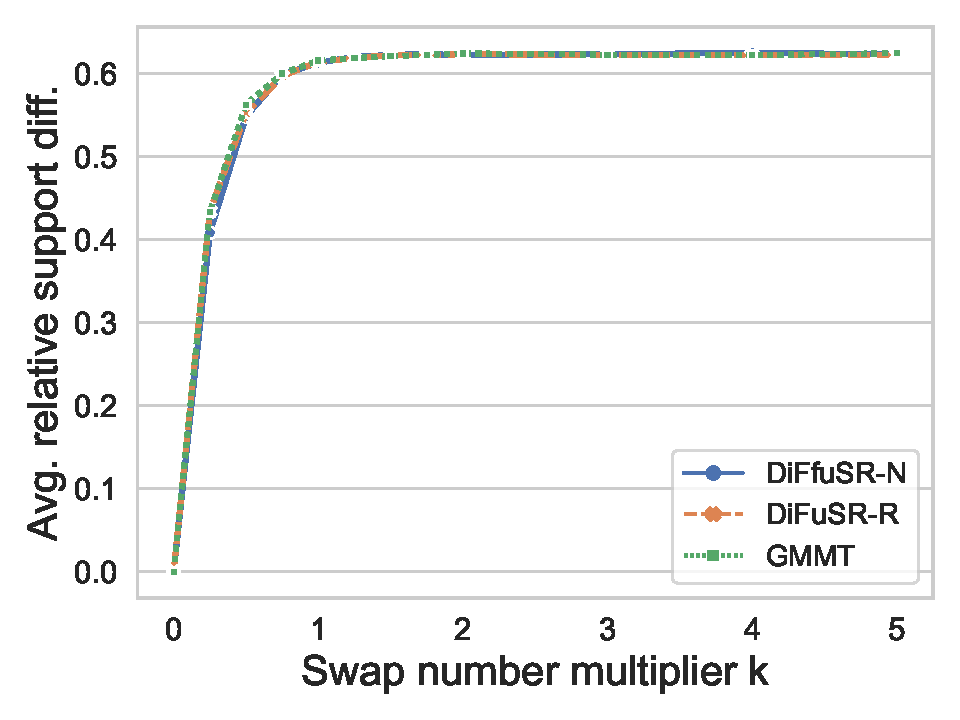
\includegraphics[width=\textwidth]{convergence-foodmart-5-0.0003-0.pdf} % chktex 8
    \caption{\textsc{Foodmart}}
  \end{subfigure}%

  \centering
  \begin{subfigure}{0.40\textwidth}
    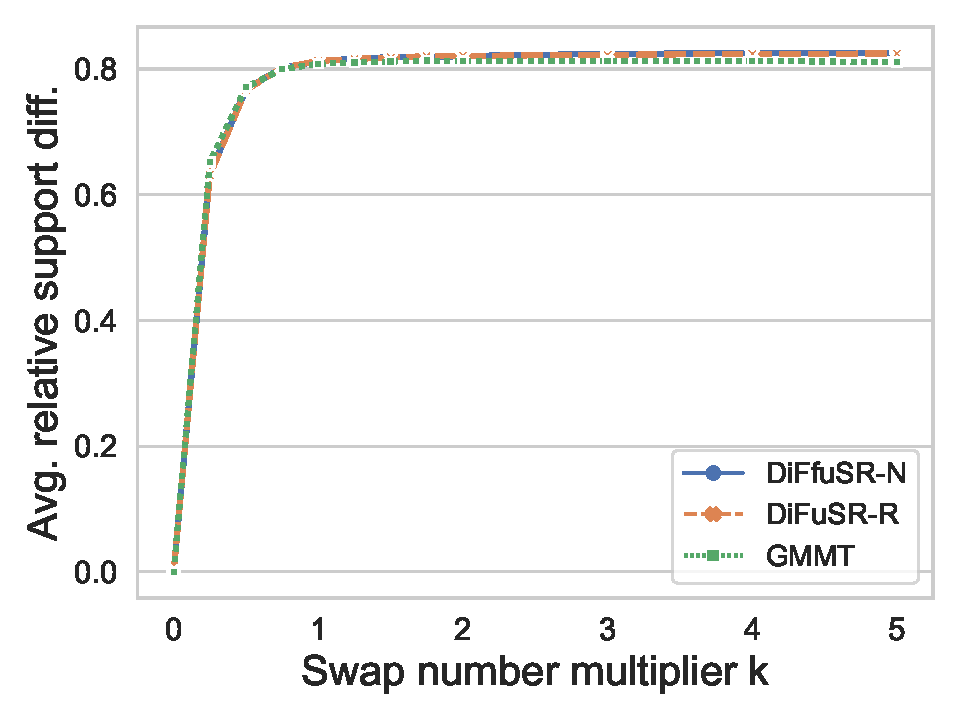
\includegraphics[width=\textwidth]{convergence-BMS2-5-0.002-0.pdf} % chktex 8
    \caption{\textsc{BMS 2}}
  \end{subfigure}
  \caption{Additional convergence results.}\label{fig:addarsd}
  \Description{Additional convergence results.}
\end{figure}


\end{document}
